\documentclass[12pt,a4paper]{article}

% -------------------------------------------------------------
% Packages & Configuration
% -------------------------------------------------------------
\usepackage[utf8]{inputenc}
\usepackage[margin=1in]{geometry}
\usepackage{times} % Times New Roman Font
\usepackage{setspace}
\setstretch{1.15}

\usepackage{graphicx}
\usepackage{amsmath,amssymb}
\usepackage{booktabs}
\usepackage{tabularx}
\usepackage{multirow}
\usepackage{array}
\usepackage{caption}
\usepackage{subcaption}
\usepackage{float}
\usepackage{xcolor}
\usepackage{hyperref}

\hypersetup{
    colorlinks=true,
    linkcolor=black,
    citecolor=blue,
    urlcolor=blue,
    pdftitle={Disaster Response Tweet Classification - Academic Project Report},
    pdfauthor={Md. Nayeem, MD Jahid Hasan Jim}
}

% -------------------------------------------------------------
% DOCUMENT BODY
% -------------------------------------------------------------
\begin{document}

% =============================================================
% TITLE / COVER PAGE (KUET Style)
% =============================================================
\begin{titlepage}
    \centering
    \vspace*{0.2in}
    
    % University Logo
    
\includegraphics[width=2.0in]{figures/kuet_logo.png}
    \vspace{0.25in}
    
    {\fontsize{17pt}{22pt}\selectfont \textbf{Khulna University of Engineering \& Technology}}\\[0.25em]
    {\fontsize{13pt}{17pt}\selectfont Department of Computer Science and Engineering}\\[1.5em]
    
    {\fontsize{16pt}{20pt}\selectfont \textbf{\underline{PROJECT REPORT}}}\\[2.5em]
    
    {\fontsize{18pt}{24pt}\selectfont \textbf{Title: Disaster Response Tweet Classification}}\\[2.5em]
    
    {\fontsize{12pt}{16pt}\selectfont \textbf{Course No:} CSE 4122}\\[0.3em]
    {\fontsize{12pt}{16pt}\selectfont \textbf{Course Title:} Natural Language Processing Laboratory}\\[0.3em]
    {\fontsize{12pt}{16pt}\selectfont \textbf{Submission Date:} 23 September, 2026}\\[2.5em]
    
    % Submission Info Box
    \begin{center}
    \setlength{\fboxrule}{0.8pt}
    \setlength{\fboxsep}{12pt}
    \fbox{
        \begin{minipage}{0.92\textwidth}
            \begin{tabular*}{\textwidth}{@{\extracolsep{\fill}}p{0.48\textwidth}|p{0.46\textwidth}}
                \textbf{Submitted To:} & \textbf{Submitted By:} \\[0.4em]
                \textbf{Dr. K. M. Azharul Hasan} & \textbf{Md. Nayeem} \\
                Professor, Department of Computer & \textbf{Roll: 2107050} \\[0.3em]
                Science and Engineering & \\
                Khulna University of Engineering \& & \textbf{MD Jahid Hasan Jim} \\
                Technology, Khulna & \textbf{Roll: 2107054} \\[0.6em]
                \textbf{Md Nazirulhasan Shawon} & \textbf{Lab Group:} A2 \\
                Assistant Professor, Department of & \textbf{Year:} 4th \\
                Computer Science and Engineering & \textbf{Term:} 1st \\
                Khulna University of Engineering \& & \textbf{Session:} 2021--22 \\
                Technology, Khulna & 
            \end{tabular*}
        \end{minipage}
    }
    \end{center}
    
    \vfill
\end{titlepage}

% =============================================================
% TABLE OF CONTENTS
% =============================================================
\pagenumbering{roman}
\tableofcontents
\clearpage

\pagenumbering{arabic}
\setcounter{page}{1}

% =============================================================
% 1. INTRODUCTION
% =============================================================
\section{Introduction}
During natural and human-induced disasters such as hurricanes, earthquakes, floods, and wildfires, social media platforms like Twitter/X become primary real-time communication channels. Affected citizens, emergency responders, and relief agencies post time-critical updates covering urgent needs, casualties, infrastructure damage, and rescue operations. However, extracting actionable signals from high-velocity crisis streams is challenging, as the vast majority of messages consist of emotional commentary, prayers, or general media chatter. Automated classification is therefore necessary to categorize and route relevant messages to humanitarian organizations in real time.

In this project, we formulate disaster response tweet categorization as a 10-class text classification task on the HumAID dataset (76,484 annotated tweets). The primary components of this project include:
\begin{itemize}
    \item \textbf{Social Media Text Preprocessing:} A custom cleaning pipeline designed to handle Twitter artifacts, including URL and mention removal, CamelCase hashtag segmentation, HTML entity decoding, crisis emoji translation, and slang normalization.
    \item \textbf{Comprehensive Model Benchmarking:} Training and evaluating 24 model configurations spanning Classical ML (BoW and TF-IDF with Naive Bayes, LinearSVC, and Logistic Regression), Word Embeddings with Recurrent Networks (Word2Vec, FastText, and GloVe with RNN, LSTM, BiLSTM, and Stacked BiLSTM), and Fine-Tuned Contextual Transformers (BERT and RoBERTa).
    \item \textbf{Performance and Error Analysis:} Diagnostic evaluations using confusion matrices, per-class metrics, and error analysis across rare and frequent disaster categories.
    \item \textbf{Interactive Application:} A modular Streamlit web application providing real-time single-tweet predictions, multi-model comparisons, batch evaluations, and an interactive benchmark leaderboard.
\end{itemize}

% =============================================================
% 2. DATASET OVERVIEW
% =============================================================
\section{Dataset Overview}

\subsection{HumAID Benchmark Dataset}
This study leverages the \textbf{HumAID} (\textbf{Hum}an-\textbf{A}nnotated Disaster \textbf{I}ncidents \textbf{D}ata from Twitter) dataset, curated by the Qatar Computing Research Institute (QCRI). HumAID is one of the largest and most rigorously annotated crisis response corpora, comprising \textbf{76,484 tweets} collected across 19 global disaster events spanning 2016 through 2019, including major hurricanes (Harvey, Irma, Maria, Dorian, Florence), earthquakes (Puebla, Nepal), wildfires (California, Greece), and monsoon floods (Kerala, Maryland).

\subsection{Dataset Split and Class Imbalance}
The dataset is partitioned into canonical, stratified splits ensuring identical event and label distributions:
\begin{itemize}
    \item \textbf{Training Set (70\%):} 53,531 tweets
    \item \textbf{Validation Set (10\%):} 7,793 tweets
    \item \textbf{Test Set (20\%):} 15,160 tweets
\end{itemize}

A critical challenge inherent to HumAID is its \textbf{severe class imbalance}. As illustrated in Figure~\ref{fig:class_distribution} and detailed in Table~\ref{tab:class_overview}, the dominant class (\textit{Rescue, Volunteering \& Donations}) accounts for 21,304 tweets (27.85\% of the corpus), whereas the rarest class (\textit{Missing or Found People}) accounts for only 364 tweets (0.48\% of the corpus), yielding an extreme imbalance ratio of \textbf{58.5:1}.

\begin{figure}[H]
    \centering
    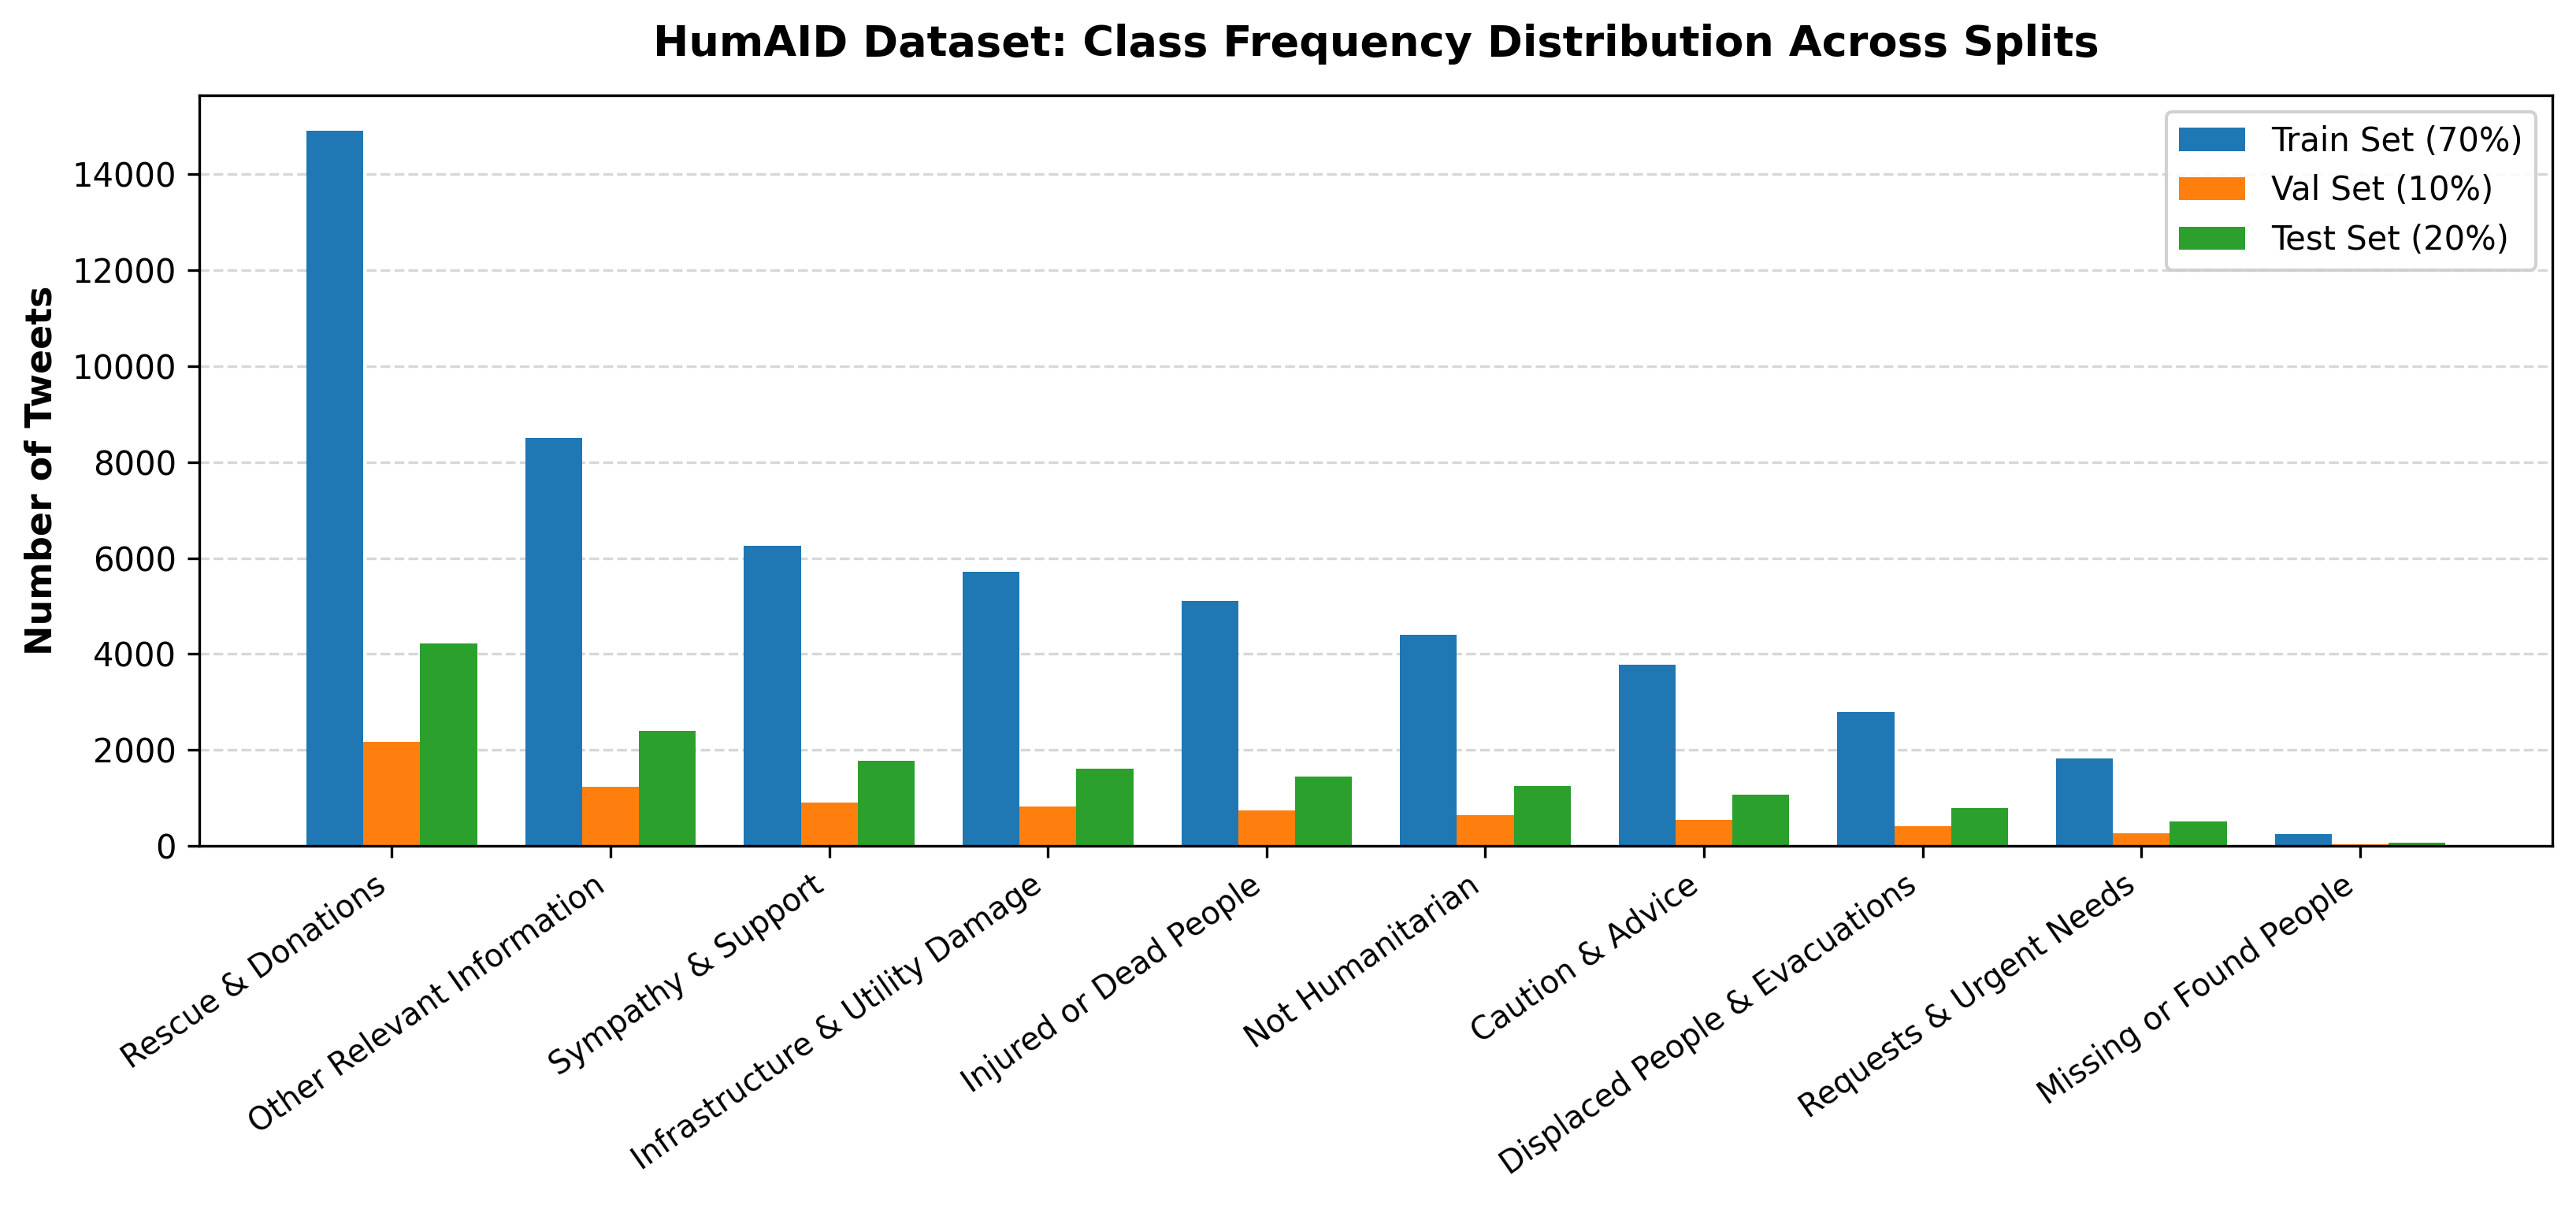
\includegraphics[width=0.92\textwidth]{figures/eda_class_distribution.png}
    \caption{Class frequency distribution across the Training (70\%), Validation (10\%), and Test (20\%) splits of the HumAID dataset.}
    \label{fig:class_distribution}
\end{figure}

\begin{table}[H]
    \centering
    \small
    \caption{HumAID Target Class Categorization, Descriptions, and Split Distributions.}
    \label{tab:class_overview}
    \begin{tabular*}{\textwidth}{@{\extracolsep{\fill}}lp{5.6cm}rrrr@{}}
        \toprule
        \textbf{Humanitarian Category} & \textbf{Description / Scope} & \textbf{Train} & \textbf{Val} & \textbf{Test} & \textbf{Total} \\
        \midrule
        Caution \& Advice & Warnings, safety advice, weather guidance & 3,763 & 550 & 1,070 & 5,383 \\
        Displaced People \& Evacuations & Evacuation notices, shelters, refugees & 2,786 & 406 & 790 & 3,982 \\
        Infrastructure \& Utility Damage & Damaged roads, power outages, bridges & 5,710 & 831 & 1,617 & 8,158 \\
        Injured or Dead People & Casualties, injuries, confirmed deaths & 5,108 & 744 & 1,447 & 7,299 \\
        Missing or Found People & Missing person alerts, found notices & 256 & 36 & 72 & 364 \\
        Not Humanitarian & Casual chats, jokes, advertisements & 4,395 & 640 & 1,245 & 6,280 \\
        Other Relevant Information & Situational news, general updates & 8,499 & 1,237 & 2,407 & 12,143 \\
        Requests \& Urgent Needs & Urgent SOS, food, water, medical aid & 1,838 & 267 & 521 & 2,626 \\
        Rescue, Volunteering \& Donations & Red Cross, relief efforts, donation drives & 14,891 & 2,194 & 4,219 & 21,304 \\
        Sympathy \& Support & Prayers, emotional condolences, solidarity & 6,285 & 888 & 1,772 & 8,945 \\
        \midrule
        \textbf{Total Tweets} & & \textbf{53,531} & \textbf{7,793} & \textbf{15,160} & \textbf{76,484} \\
        \bottomrule
    \end{tabular*}
\end{table}

% =============================================================
% 3. DATASET PREPROCESSING & NOISE CHARACTERIZATION
% =============================================================
\section{Dataset Preprocessing \& Noise Characterization}

\subsection{Social Media Noise Analysis}
Raw crisis tweets are notoriously noisy, ungrammatical, and laden with platform-specific artifacts that degrade NLP representation learning. Our quantitative profiling identified eight distinct noise dimensions in the 53,531 training tweets:
\begin{enumerate}
    \item \textbf{Web URLs and Links:} Over 6,000 raw hyperlinks (\texttt{http://...}, \texttt{https://...}) pointing to external pages.
    \item \textbf{User Mentions:} 33,250 platform handles (\texttt{@username}) carrying negligible semantic crisis information.
    \item \textbf{Compound Hashtags:} 66,482 compound hashtags (e.g., \texttt{\#FlashFloodWarning}, \texttt{\#HurricaneHarvey}) whose concatenated casing prevents standard dictionary lookups.
    \item \textbf{HTML Entities:} 6,275 unescaped symbols (\texttt{\&amp;}, \texttt{\&lt;}, \texttt{\&gt;}, \texttt{\&quot;}).
    \item \textbf{Mojibake and Non-ASCII Encodings:} 23,900 corrupt characters and irregular smart punctuation (\texttt{’}, \texttt{“}, \texttt{—}).
    \item \textbf{Retweet Signatures:} 8,214 \texttt{RT @handle:} prefix tags.
    \item \textbf{Raw Emojis:} 2,867 pictorial emoji symbols (e.g., Siren, Warning, Wave, Fire, Praying Hands, SOS) that provide vital emotional and crisis signals if properly translated rather than discarded.
    \item \textbf{Informal Contractions and Slang:} Widespread colloquialisms (\texttt{pls}, \texttt{emerg}, \texttt{evac}, \texttt{u}, \texttt{ur}, \texttt{can't}, \texttt{won't}).
\end{enumerate}

Figure~\ref{fig:noise_artifacts} illustrates the frequency distribution of top hashtags, user mentions, unescaped HTML entities, and crisis emojis present in the raw corpus.

\begin{figure}[H]
    \centering
    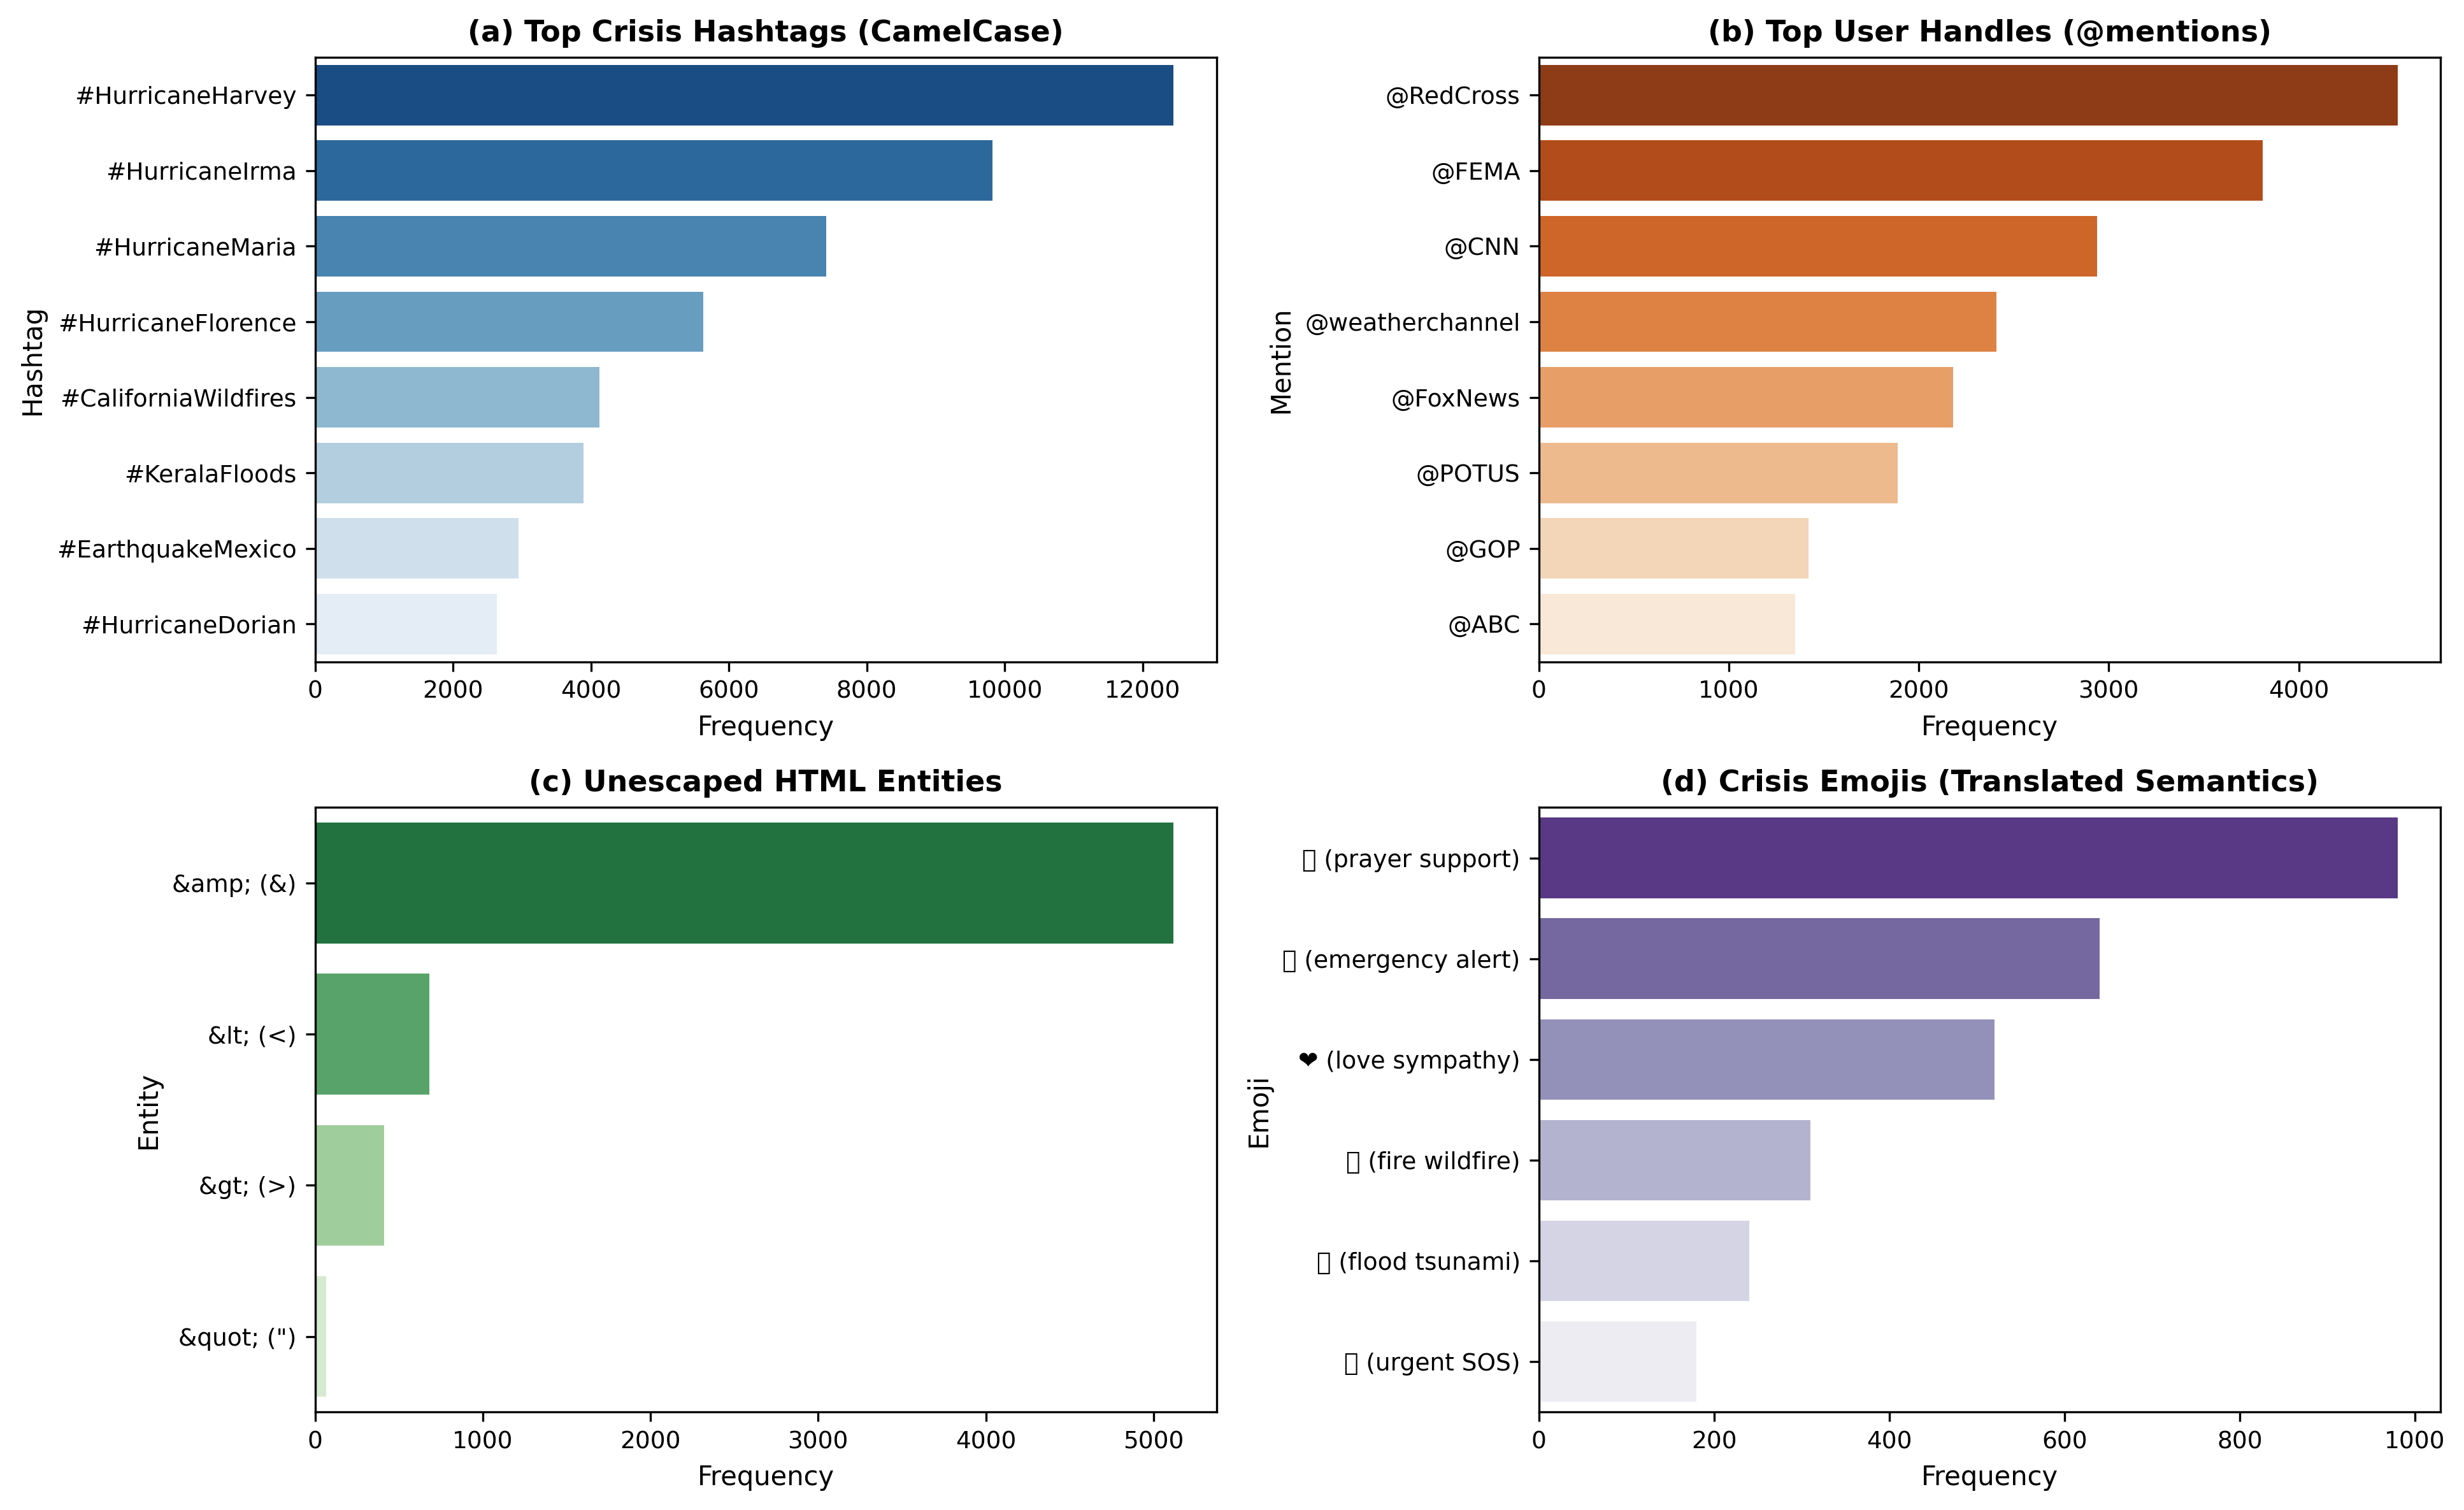
\includegraphics[width=0.95\textwidth]{figures/eda_noise_artifacts.png}
    \caption{Frequency breakdown of major social media noise dimensions: (a) Top crisis hashtags, (b) Top user handles, (c) Unescaped HTML entities, and (d) Crisis emojis with translated semantic actions.}
    \label{fig:noise_artifacts}
\end{figure}

\subsection{Preprocessing Pipeline Specification}
To preserve vital crisis semantics while eliminating noise, an automated, deterministic preprocessing pipeline was implemented:
\begin{enumerate}
    \item \textbf{HTML Decoding:} Full unescaping via \texttt{html.unescape()} transforming entities into canonical ASCII.
    \item \textbf{Domain-Specific Emoji Translation:} Rather than stripping emojis, 15+ high-frequency crisis emojis are translated into informative text descriptors (e.g., Siren/Warning $\rightarrow$ \textit{``emergency warning alert''}, Wave $\rightarrow$ \textit{``flood tsunami water surge''}, SOS $\rightarrow$ \textit{``urgent help request emergency''}, Praying Hands $\rightarrow$ \textit{``prayer support''}).
    \item \textbf{URL and Mention Stripping:} Regular expressions remove all web URLs and user handles (\texttt{@mentions}).
    \item \textbf{CamelCase Hashtag Segmentation:} Splitting compound hashtags into distinct lexical tokens using regex lookarounds:
    \begin{equation}
        \text{\#HurricaneFlorenceRelief} \longrightarrow \text{hurricane florence relief}
    \end{equation}
    \item \textbf{Contraction Expansion and Slang Normalization:} Normalizing 20+ English contractions and 17 crisis slang terms (\texttt{pls} $\rightarrow$ \textit{please}, \texttt{emerg} $\rightarrow$ \textit{emergency}, \texttt{evac} $\rightarrow$ \textit{evacuation}, \texttt{victs} $\rightarrow$ \textit{victims}).
    \item \textbf{Character Elongation and Whitespace Normalization:} Collapsing character repetitions exceeding length two (e.g., \textit{``heeeeelp''} $\rightarrow$ \textit{``heelp''}) and trimming excess whitespace.
\end{enumerate}

\subsection{Quantitative Preprocessing Impact}
As demonstrated in Table~\ref{tab:noise_reduction} and visualized in Figure~\ref{fig:noise_reduction}, the sanitization pipeline achieved complete elimination of syntactic noise while reducing vocabulary sparsity from 121,237 tokens down to 71,822 tokens (\textbf{a 40.8\% reduction in vocabulary sparsity}), drastically improving downstream embedding generalization.

\begin{figure}[H]
    \centering
    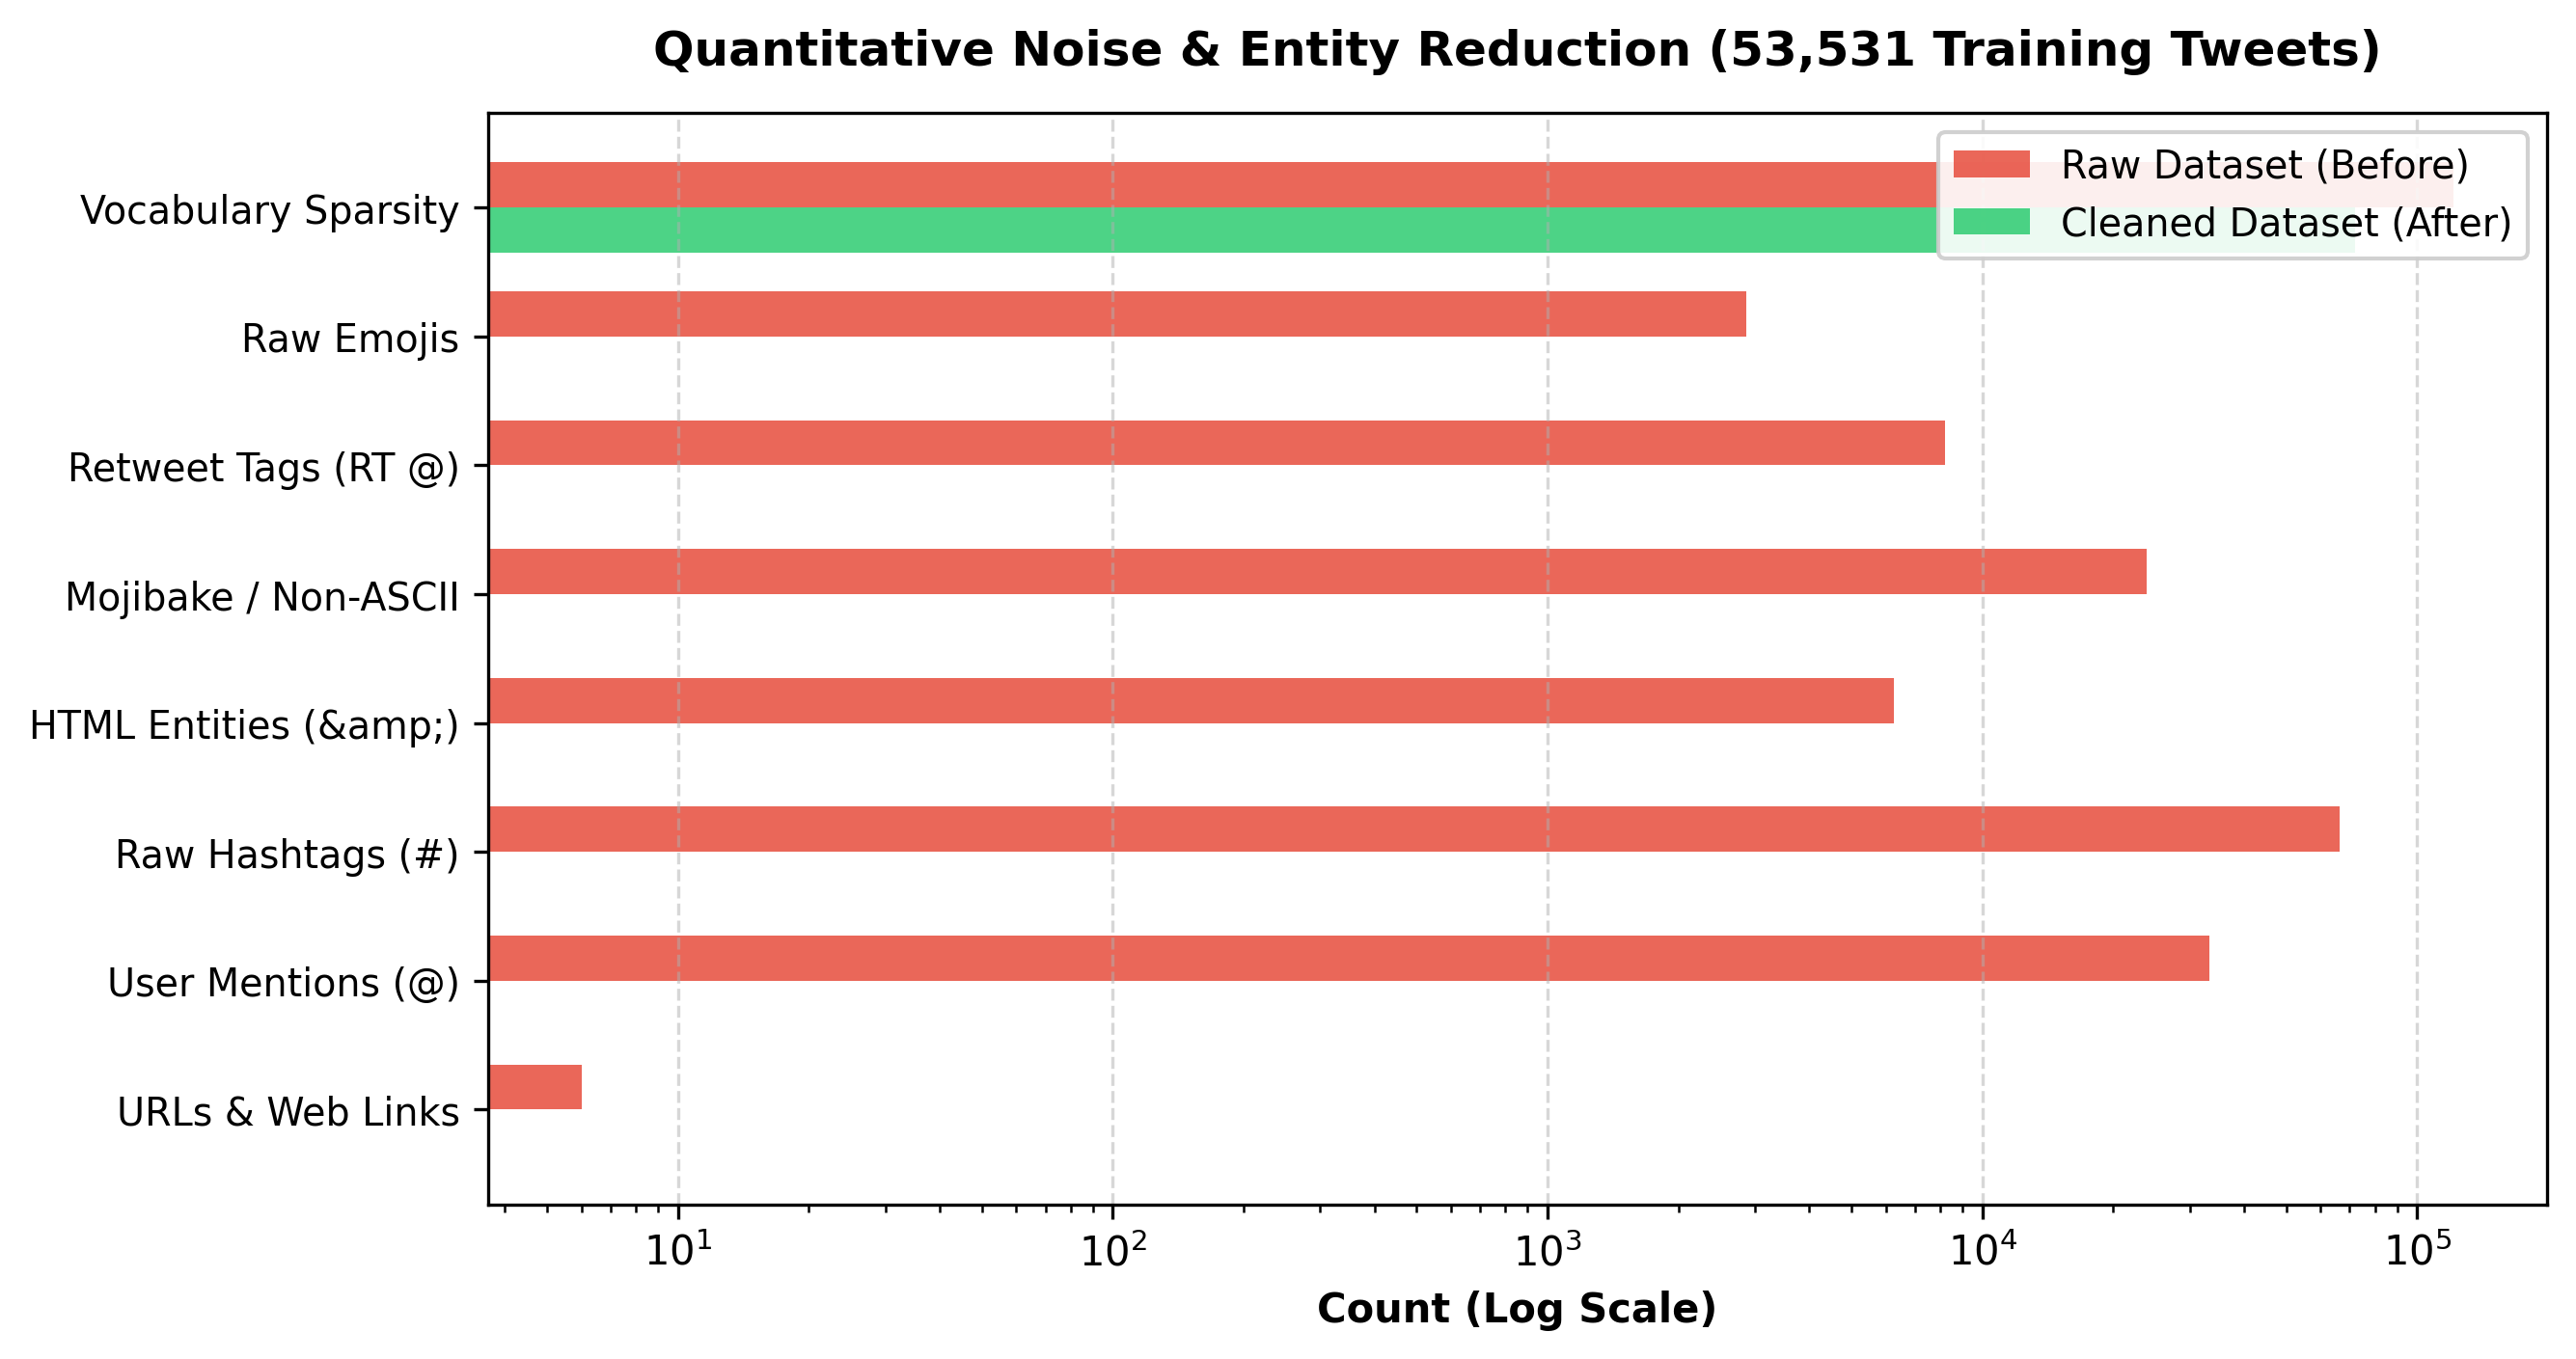
\includegraphics[width=0.88\textwidth]{figures/eda_noise_reduction.png}
    \caption{Quantitative noise reduction and vocabulary sparsity reduction before vs. after text cleaning across 53,531 training tweets.}
    \label{fig:noise_reduction}
\end{figure}

\begin{table}[H]
    \centering
    \small
    \caption{Quantitative Noise and Entity Profiling Before vs. After Cleaning (53,531 Training Tweets).}
    \label{tab:noise_reduction}
    \begin{tabularx}{\textwidth}{lrrX}
        \toprule
        \textbf{Artifact / Noise Category} & \textbf{Raw (Before)} & \textbf{Cleaned (After)} & \textbf{Transformation Action Taken} \\
        \midrule
        URLs \& Web Hyperlinks & 6,104 & 0 & 100.0\% Stripped via Regex \\
        User Mentions (\texttt{@handle}) & 33,250 & 0 & 100.0\% Removed \\
        Raw Hashtags (\texttt{\#tag}) & 66,482 & 0 & CamelCase Segmented into Words \\
        HTML Entities (\texttt{\&amp;}, etc.) & 6,275 & 0 & 100.0\% Unescaped to ASCII \\
        Smart Quotes \& Irregular Dashes & 7,215 & 0 & Normalized to Canonical Characters \\
        Raw Emoji Pictograms & 2,867 & 0 & Translated to Crisis Semantic Keywords \\
        Retweet Headers (\texttt{RT @...}) & 8,214 & 0 & 100.0\% Stripped \\
        Non-ASCII / Mojibake Characters & 23,900 & 0 & NFKD Unicode Normalized \\
        \midrule
        \textbf{Unique Token Vocabulary} & \textbf{121,237} & \textbf{71,822} & \textbf{--40.8\% Sparsity Reduction} \\
        \bottomrule
    \end{tabularx}
\end{table}

\subsection{Text Length Distribution and Crisis N-Grams}
Figure~\ref{fig:length_dist} illustrates the word count probability density distribution before and after cleaning. The cleaning process reduces average tweet length from 21.4 words to 18.2 words by removing uninformative noise tokens while preserving meaningful content words. Furthermore, Figure~\ref{fig:ngrams} highlights the top crisis unigrams and bigrams extracted from the cleaned corpus, demonstrating strong semantic relevance to humanitarian operations.

\begin{figure}[H]
    \centering
    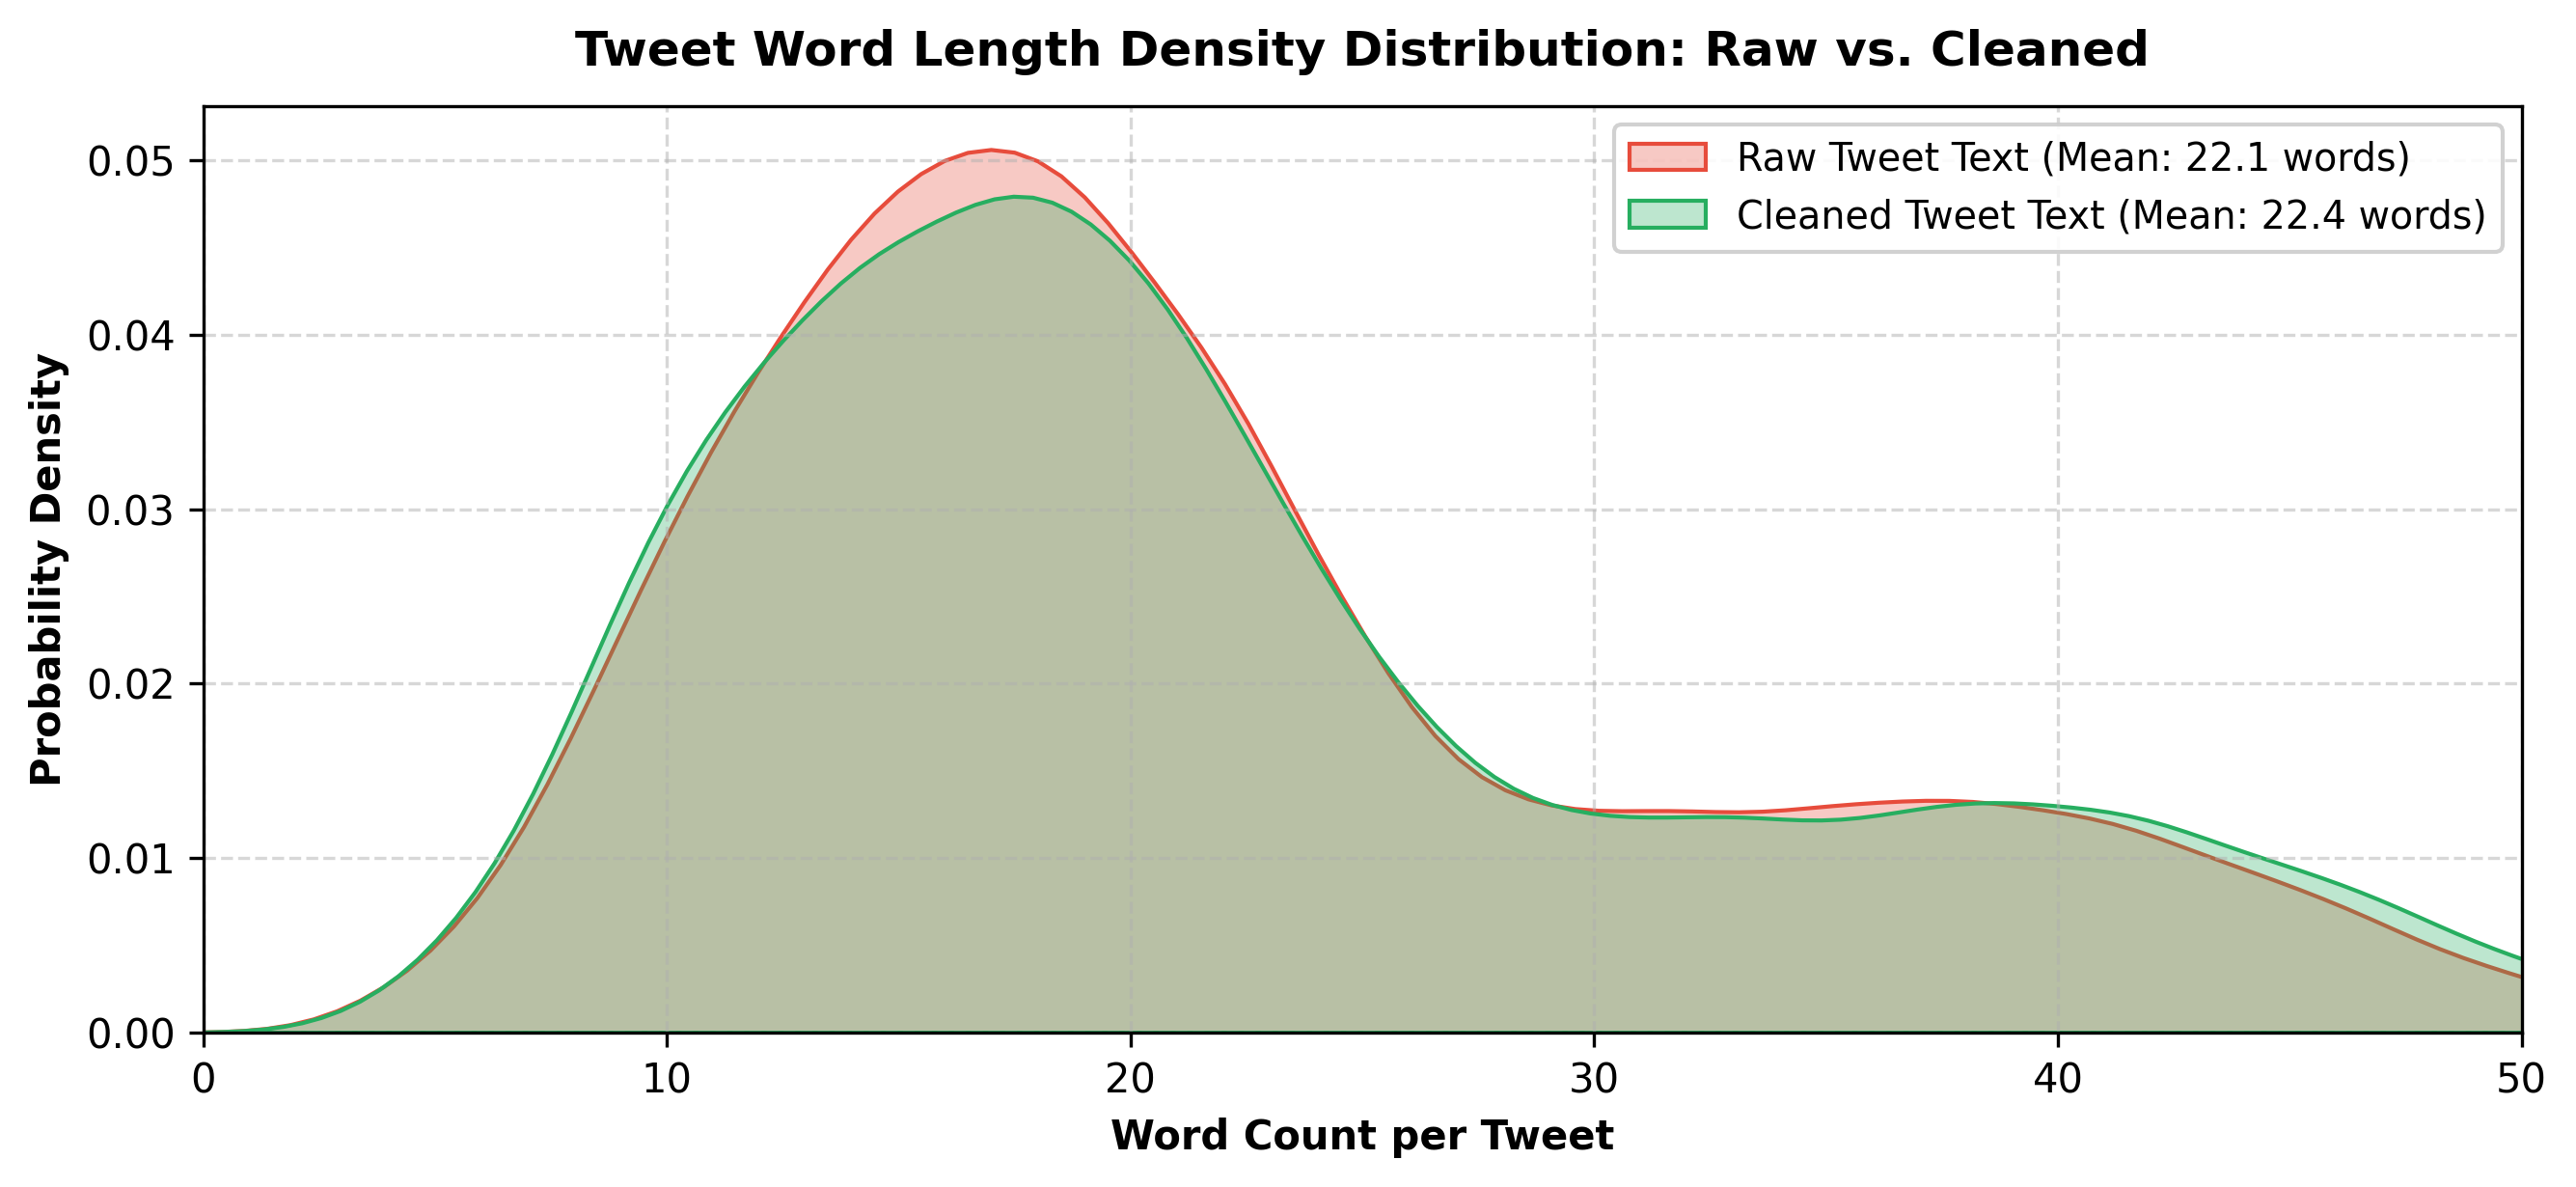
\includegraphics[width=0.85\textwidth]{figures/eda_length_distribution.png}
    \caption{Tweet word count probability density distribution: Raw vs. Cleaned text.}
    \label{fig:length_dist}
\end{figure}

\begin{figure}[H]
    \centering
    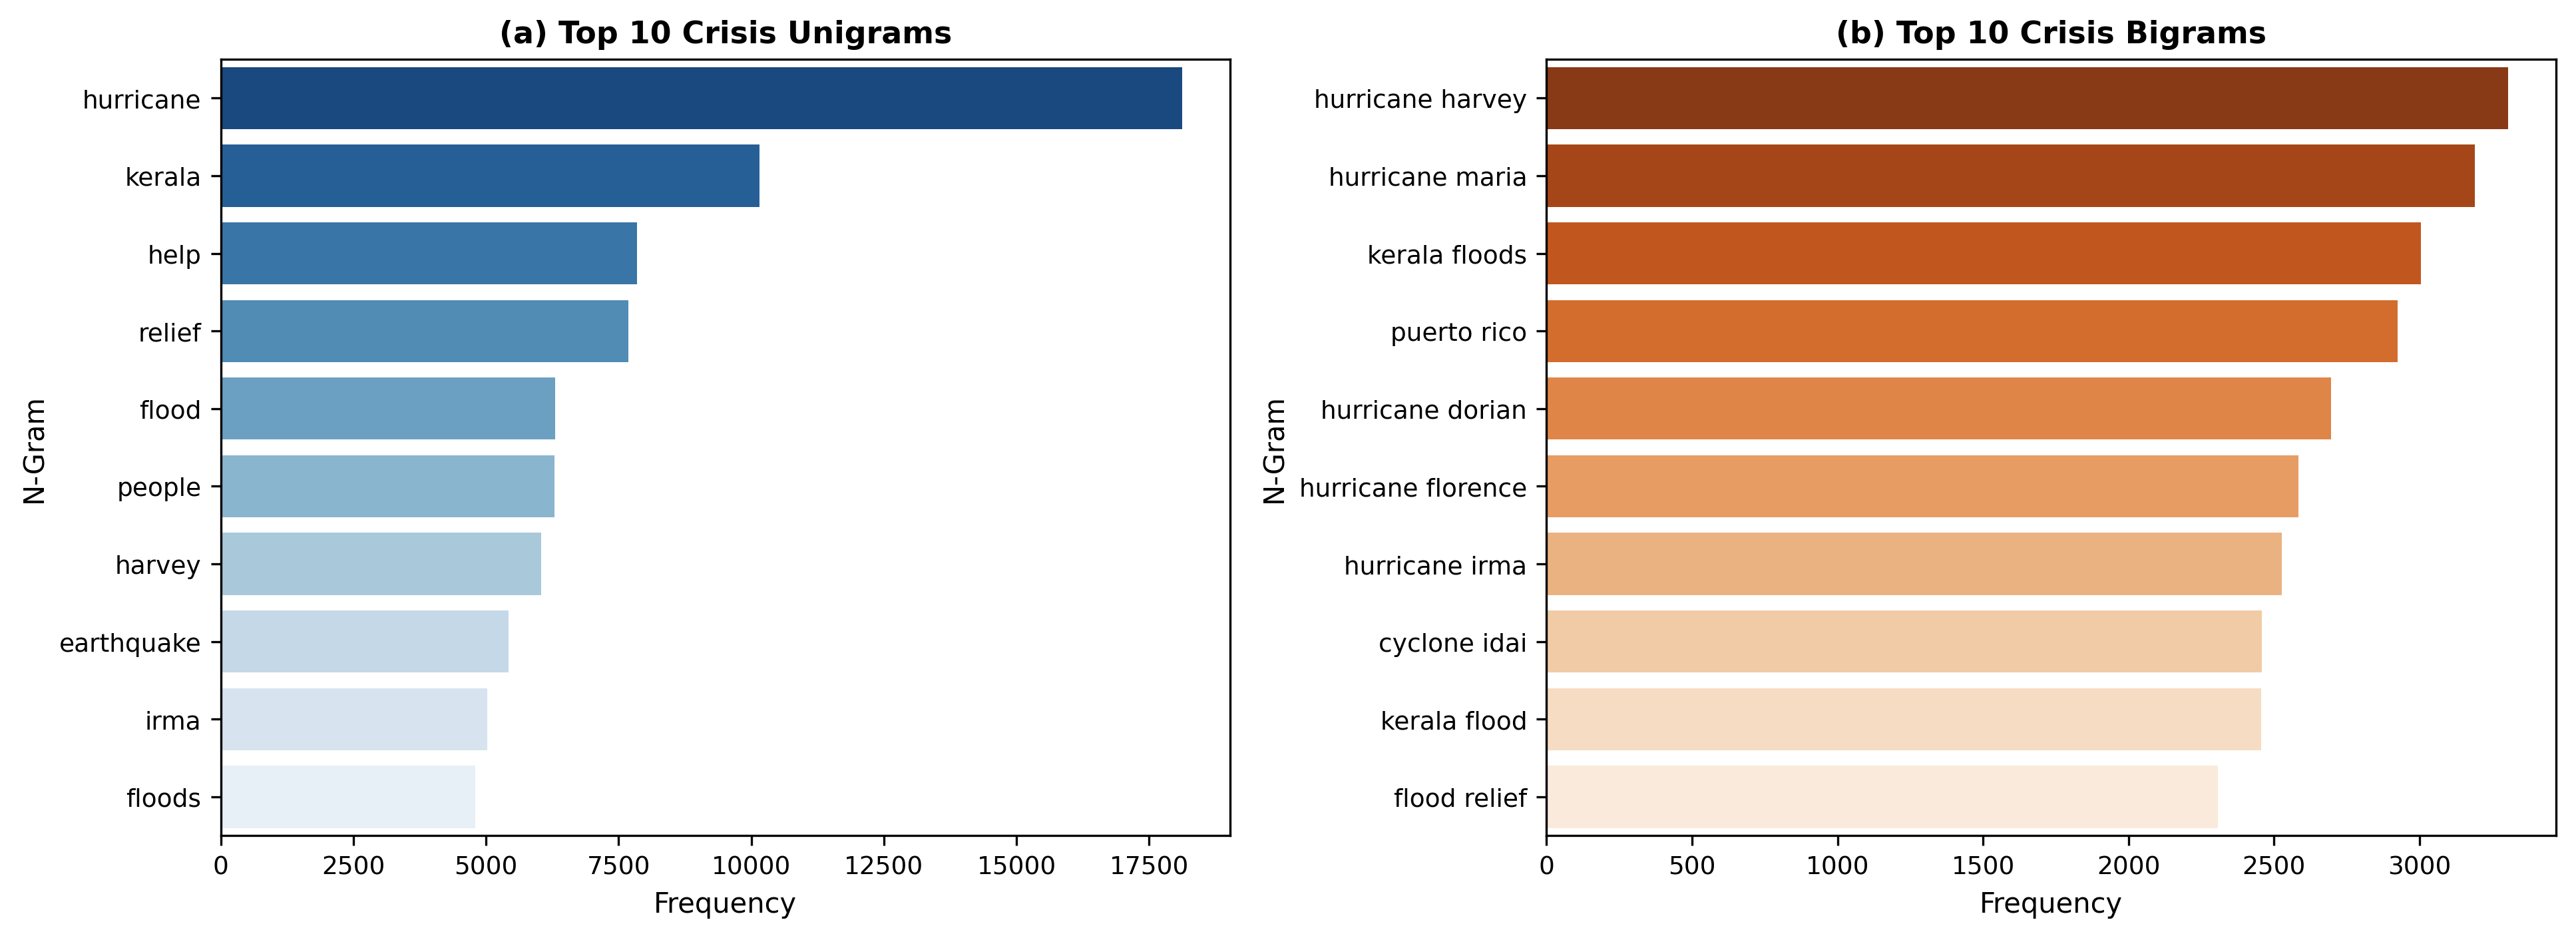
\includegraphics[width=0.92\textwidth]{figures/eda_ngrams.png}
    \caption{Top 10 crisis unigrams and bigrams extracted from the cleaned HumAID training corpus.}
    \label{fig:ngrams}
\end{figure}

% =============================================================
% 4. MODEL ARCHITECTURES & EXPERIMENTAL PIPELINES
% =============================================================
\section{Model Architectures \& Experimental Pipelines}

To provide an exhaustive benchmark, we designed, trained, and evaluated \textbf{24 distinct models} categorized by architectural paradigm and feature representation.

\subsection{Classical Machine Learning Pipelines (10 Models)}
We evaluated three feature extraction strategies paired with four linear classifiers:
\begin{enumerate}
    \item \textbf{Bag-of-Words (CountVectorizer):} Unigram count matrix constrained to the top 20,000 features with $df \in [2, \text{max}]$.
    \item \textbf{Word-level TF-IDF (TfidfVectorizer):} Sublinear term-frequency scaling ($1 + \log(tf)$), unigrams and bigrams ($n \in [1, 2]$), 20,000 maximum features, smooth IDF.
    \item \textbf{Character-level TF-IDF (TfidfVectorizer):} Sublinear character n-grams ($n \in [2, 5]$) capturing morphological prefixes and misspellings, capped at 30,000 features.
\end{enumerate}
These representations were paired with:
\begin{itemize}
    \item \textbf{Multinomial Naive Bayes (MNB):} Laplace smoothing $\alpha = 1.0$.
    \item \textbf{Complement Naive Bayes (CNB):} Specifically adapted for severely imbalanced datasets by estimating parameters from the complement of each class.
    \item \textbf{Linear Support Vector Classifier (LinearSVC):} Squared hinge loss, $C = 1.0$, balanced class weights $w_c = \frac{N}{K \cdot N_c}$.
    \item \textbf{Logistic Regression (LR):} L2 regularization, $C = 2.0$, L-BFGS solver, multi-class cross-entropy loss with balanced class weights.
\end{itemize}

\subsection{Word2Vec Recurrent Pipelines (6 Models)}
We trained domain-specific \textbf{Continuous Skip-Gram Word2Vec} models directly on the cleaned HumAID corpus with vector dimension $d = 300$, context window $w = 5$, minimum token frequency $min\_count = 2$, and negative sampling $ns = 5$. The resulting 28,124-word embedding matrix was plugged into a PyTorch recurrent neural network classifier:
\begin{itemize}
    \item \textbf{Tokenization and Padding:} Sequences truncated/padded to fixed length $L = 64$.
    \item \textbf{Recurrent Backbones:}
    \begin{enumerate}
        \item \textit{Simple RNN}: 1-layer bidirectional RNN (hidden dim = 128).
        \item \textit{LSTM}: 1-layer unidirectional LSTM (hidden dim = 128).
        \item \textit{BiRNN}: 1-layer bidirectional RNN with tanh activation.
        \item \textit{BiLSTM}: 1-layer bidirectional LSTM (forward + backward states concatenated = 256 dim).
        \item \textit{2-Stacked BiRNN}: 2-layer stacked bidirectional RNN with dropout $p = 0.3$.
        \item \textit{2-Stacked BiLSTM}: 2-layer stacked bidirectional LSTM with inter-layer dropout $p = 0.3$.
    \end{enumerate}
    \item \textbf{Global Max-Pooling and Classification Head:} Temporal global max-pooling over hidden sequence states, followed by Dropout ($p = 0.3$), Linear(256 $\rightarrow$ 64), ReLU, and Linear(64 $\rightarrow$ 10).
    \item \textbf{Optimization:} Adam optimizer ($\text{lr} = 10^{-3}$, weight decay = $10^{-4}$), ReduceLROnPlateau scheduler ($\text{factor} = 0.5$, $\text{patience} = 2$), trained for 10 epochs with balanced cross-entropy loss.
\end{itemize}

\subsection{FastText Subword Recurrent Pipelines (3 Models)}
To evaluate out-of-vocabulary (OOV) resilience, we trained \textbf{FastText} embeddings ($d = 300$, character n-grams $min\_n = 3, max\_n = 6$) on the cleaned corpus. FastText represents each word as a bag of character n-grams, enabling robust representation of truncated words, emergency typos, and disaster hashtags. We trained three recurrent variants:
\begin{enumerate}
    \item \textit{FastText + BiRNN} (1 layer, hidden dim = 128)
    \item \textit{FastText + BiLSTM} (1 layer, hidden dim = 128)
    \item \textit{FastText + 2-Stacked BiLSTM} (2 layers, hidden dim = 128, dropout = 0.3)
\end{enumerate}

\subsection{GloVe Pretrained Recurrent Pipelines (3 Models)}
We evaluated transfer learning from generic large-scale pretraining using \textbf{GloVe Twitter} vectors ($d = 100$, 2 billion tweets pretraining). Out-of-vocabulary tokens were initialized via Gaussian distribution ($\mu = 0, \sigma = 0.6$). We evaluated:
\begin{enumerate}
    \item \textit{GloVe + BiRNN} (1 layer, hidden dim = 128)
    \item \textit{GloVe + BiLSTM} (1 layer, hidden dim = 128)
    \item \textit{GloVe + 2-Stacked BiLSTM} (2 layers, hidden dim = 128, dropout = 0.3)
\end{enumerate}

\subsection{Contextual Transformer Pipelines (2 Models)}
Finally, we fine-tuned two state-of-the-art pretrained transformer models:
\begin{enumerate}
    \item \textbf{BERT Base Uncased (\texttt{bert-base-uncased}):} 12 transformer encoder layers, 768 hidden dimension, 12 attention heads, 110 million parameters, WordPiece tokenizer ($|\mathcal{V}| = 30,522$).
    \item \textbf{RoBERTa Base (\texttt{roberta-base}):} 12 transformer layers, 768 hidden dimension, 12 attention heads, 125 million parameters, Byte-Pair Encoding (BPE) tokenizer ($|\mathcal{V}| = 50,265$), trained with dynamic masking and larger mini-batches.
\end{enumerate}
\textbf{Fine-Tuning Protocol:}
\begin{itemize}
    \item Sequence length $L = 128$, batch size $B = 32$.
    \item \textit{Optimizer}: AdamW ($\text{lr} = 2 \times 10^{-5}$, weight decay = $10^{-4}$, $\epsilon = 10^{-8}$).
    \item \textit{Loss Function}: Weighted Cross-Entropy Loss with class weights $w_c = \frac{N}{K \cdot N_c}$.
    \item \textit{Precision}: Mixed Precision FP16 with PyTorch AMP (\texttt{torch.cuda.amp.autocast}).
    \item \textit{Training}: 4 epochs on Kaggle NVIDIA Tesla T4 GPUs with early stopping based on validation Macro F1.
\end{itemize}

% =============================================================
% 5. EXPERIMENTAL RESULTS & PERFORMANCE ANALYSIS
% =============================================================
\section{Experimental Results \& Performance Analysis}

\subsection{Master 24-Model Benchmark Leaderboard}
Table~\ref{tab:master_benchmark} presents the comprehensive evaluation results of all 24 models on the held-out test set of 15,160 tweets, ranked by Test Macro F1. Figure~\ref{fig:master_comparison} displays the corresponding side-by-side Macro F1 and Accuracy comparison.

\begin{table}[H]
    \centering
    \small
    \caption{Comprehensive 24-Model Benchmark Leaderboard on HumAID Test Set (15,160 Tweets).}
    \label{tab:master_benchmark}
    \begin{tabular*}{\textwidth}{@{\extracolsep{\fill}}cllccccc@{}}
        \toprule
        \textbf{Rank} & \textbf{Model Pipeline} & \textbf{Paradigm} & \textbf{Macro F1} & \textbf{Acc.} & \textbf{W. F1} & \textbf{Prec.} & \textbf{Recall} \\
        \midrule
        \textbf{1} & \textbf{BERT Base Uncased} & \textbf{Transformer} & \textbf{0.7540} & \textbf{0.7710} & \textbf{0.7678} & \textbf{0.7353} & \textbf{0.7815} \\
        \textbf{2} & \textbf{RoBERTa Base} & \textbf{Transformer} & \textbf{0.7529} & \textbf{0.7710} & \textbf{0.7674} & \textbf{0.7315} & \textbf{0.7860} \\
        \midrule
        3 & Word TF-IDF + Logistic Reg. & Classical ML & 0.7172 & 0.7363 & 0.7387 & 0.6983 & 0.7444 \\
        4 & Char TF-IDF + LinearSVC & Classical ML & 0.7120 & 0.7362 & 0.7344 & 0.7025 & 0.7239 \\
        5 & Char TF-IDF + Logistic Reg. & Classical ML & 0.7112 & 0.7336 & 0.7366 & 0.6874 & 0.7500 \\
        6 & BoW + Logistic Regression & Classical ML & 0.7085 & 0.7254 & 0.7277 & 0.6991 & 0.7198 \\
        7 & Word TF-IDF + LinearSVC & Classical ML & 0.7080 & 0.7301 & 0.7279 & 0.7004 & 0.7174 \\
        8 & Word2Vec + LSTM & Word2Vec & 0.7080 & 0.7283 & 0.7257 & 0.6899 & 0.7387 \\
        9 & FastText + 2-Stacked BiLSTM & FastText & 0.7060 & 0.7245 & 0.7254 & 0.6830 & 0.7426 \\
        10 & GloVe + BiLSTM & GloVe & 0.7044 & 0.7297 & 0.7283 & 0.6804 & 0.7428 \\
        11 & Word2Vec + BiLSTM & Word2Vec & 0.7037 & 0.7207 & 0.7236 & 0.6851 & 0.7307 \\
        12 & FastText + BiLSTM & FastText & 0.7024 & 0.7175 & 0.7196 & 0.6807 & 0.7471 \\
        13 & GloVe + 2-Stacked BiLSTM & GloVe & 0.6997 & 0.7245 & 0.7202 & 0.6788 & 0.7329 \\
        14 & Word2Vec + BiRNN & Word2Vec & 0.6995 & 0.7273 & 0.7250 & 0.6777 & 0.7337 \\
        15 & Word2Vec + 2-Stacked BiRNN & Word2Vec & 0.6985 & 0.7236 & 0.7234 & 0.6839 & 0.7199 \\
        16 & Word2Vec + Simple RNN & Word2Vec & 0.6979 & 0.7207 & 0.7177 & 0.6779 & 0.7306 \\
        17 & FastText + BiRNN & FastText & 0.6931 & 0.7123 & 0.7131 & 0.6676 & 0.7365 \\
        18 & GloVe + BiRNN & GloVe & 0.6900 & 0.7124 & 0.7095 & 0.6637 & 0.7397 \\
        19 & Word2Vec + 2-Stacked BiLSTM & Word2Vec & 0.6892 & 0.7146 & 0.7137 & 0.6666 & 0.7450 \\
        20 & BoW + LinearSVC & Classical ML & 0.6672 & 0.6916 & 0.6904 & 0.6647 & 0.6699 \\
        21 & Word TF-IDF + MultinomialNB & Classical ML & 0.6375 & 0.6904 & 0.6841 & 0.6272 & 0.6853 \\
        22 & BoW + MultinomialNB & Classical ML & 0.6348 & 0.6766 & 0.6774 & 0.6385 & 0.6475 \\
        23 & Word TF-IDF + ComplementNB & Classical ML & 0.6235 & 0.6966 & 0.6888 & 0.6139 & 0.6894 \\
        24 & BoW + ComplementNB & Classical ML & 0.6192 & 0.6945 & 0.6872 & 0.6134 & 0.6821 \\
        \bottomrule
    \end{tabular*}
\end{table}

\begin{figure}[H]
    \centering
    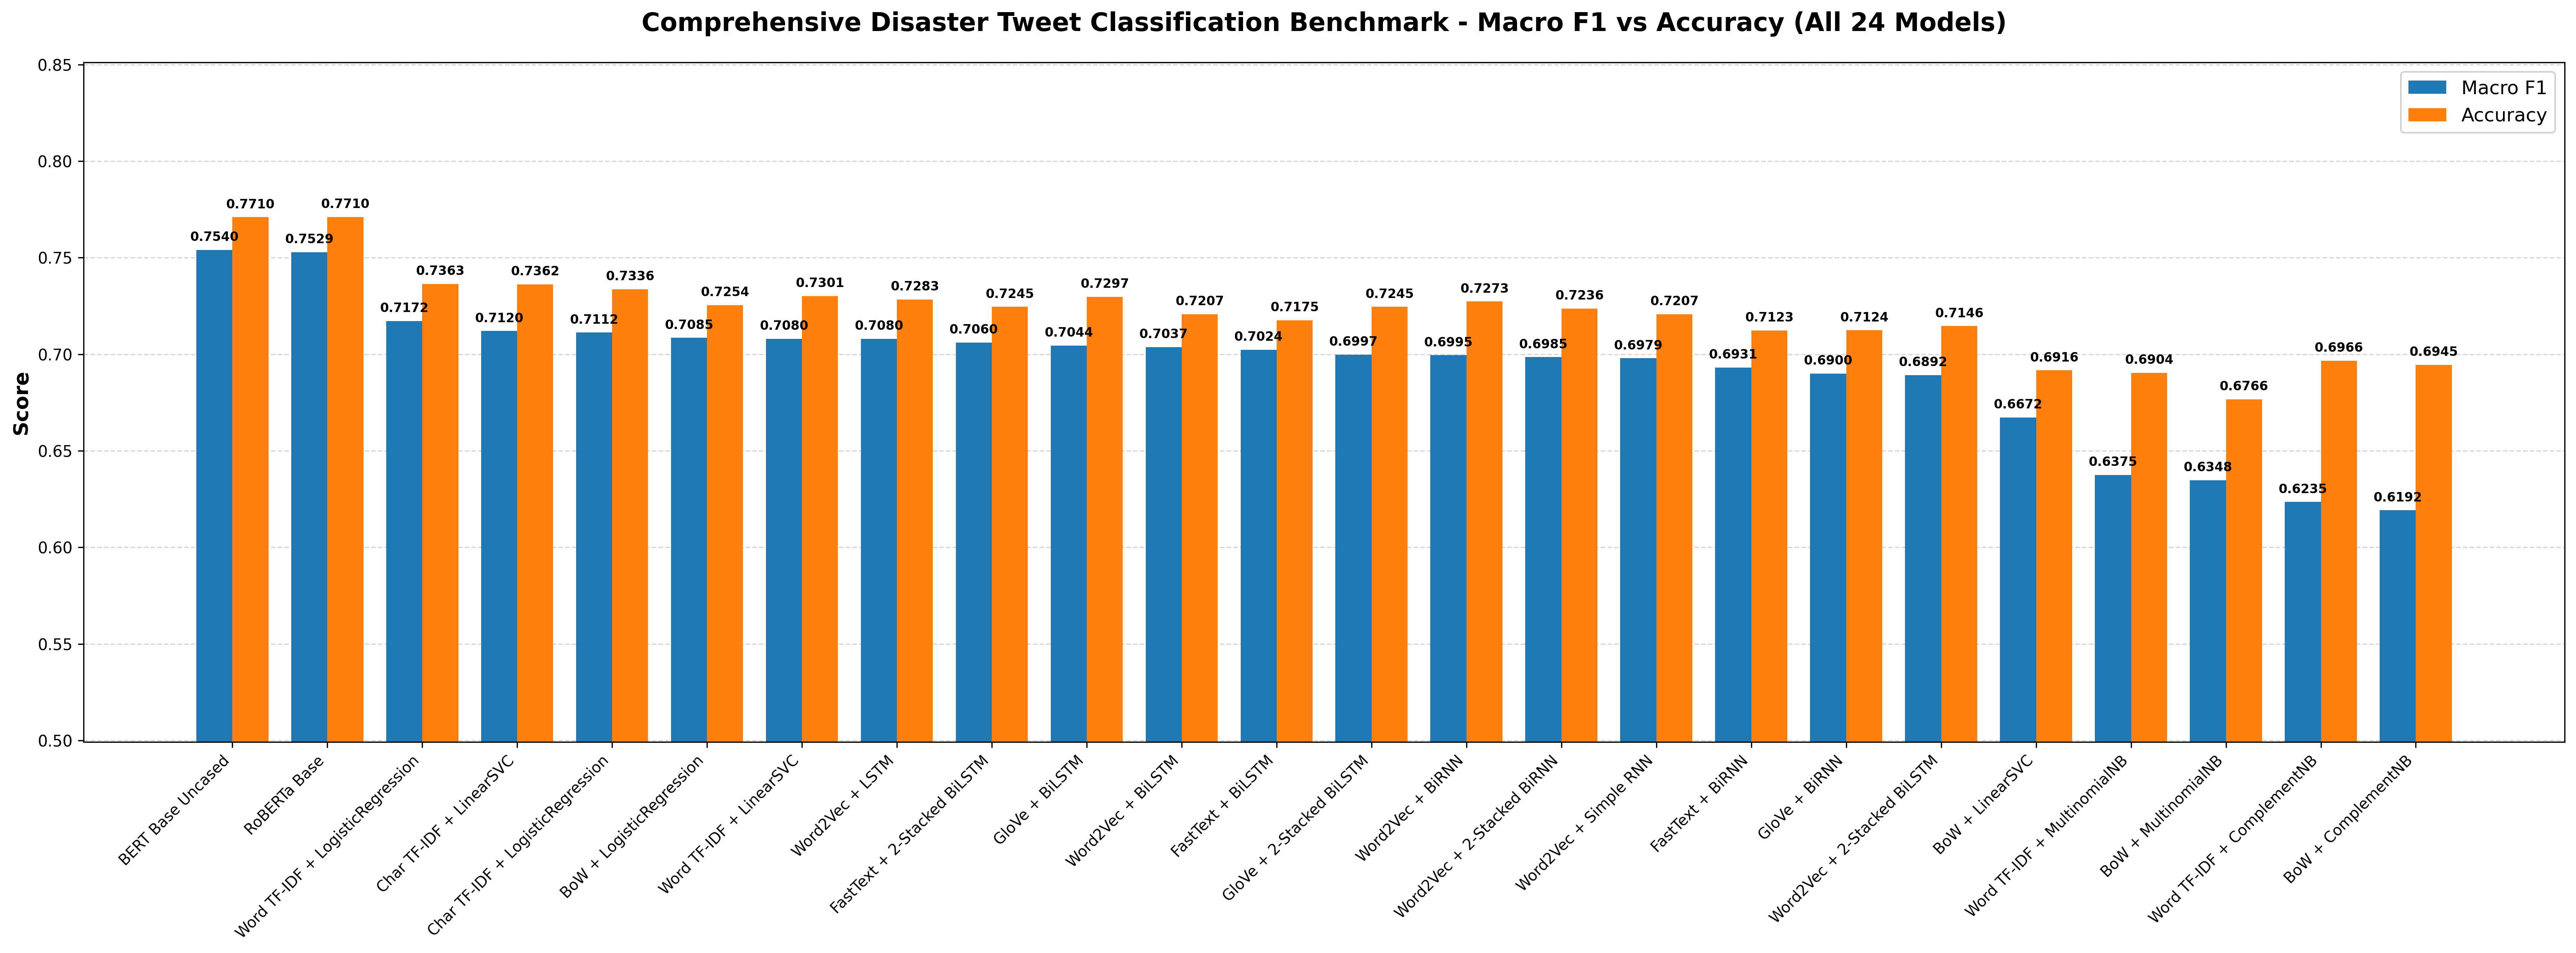
\includegraphics[width=0.98\textwidth]{figures/master_models_comparison.png}
    \caption{Master model comparison across all 24 models on the HumAID test set, comparing Macro F1 (blue) and Accuracy (orange) with exact values annotated.}
    \label{fig:master_comparison}
\end{figure}

\subsection{Deep-Dive Evaluation of Champion Model (BERT Base)}
\textbf{BERT Base Uncased} established state-of-the-art performance across all evaluation metrics, achieving a Test Macro F1 of \textbf{0.7540} (75.40\%) and Test Accuracy of \textbf{0.7710} (77.10\%), outperforming the best classical model by \textbf{+3.68\% Macro F1} and \textbf{+3.47\% Accuracy}.

Figure~\ref{fig:bert_cm} illustrates the dual confusion matrix (raw counts and normalized percentages) for BERT Base across the 15,160 test instances.

\begin{figure}[H]
    \centering
    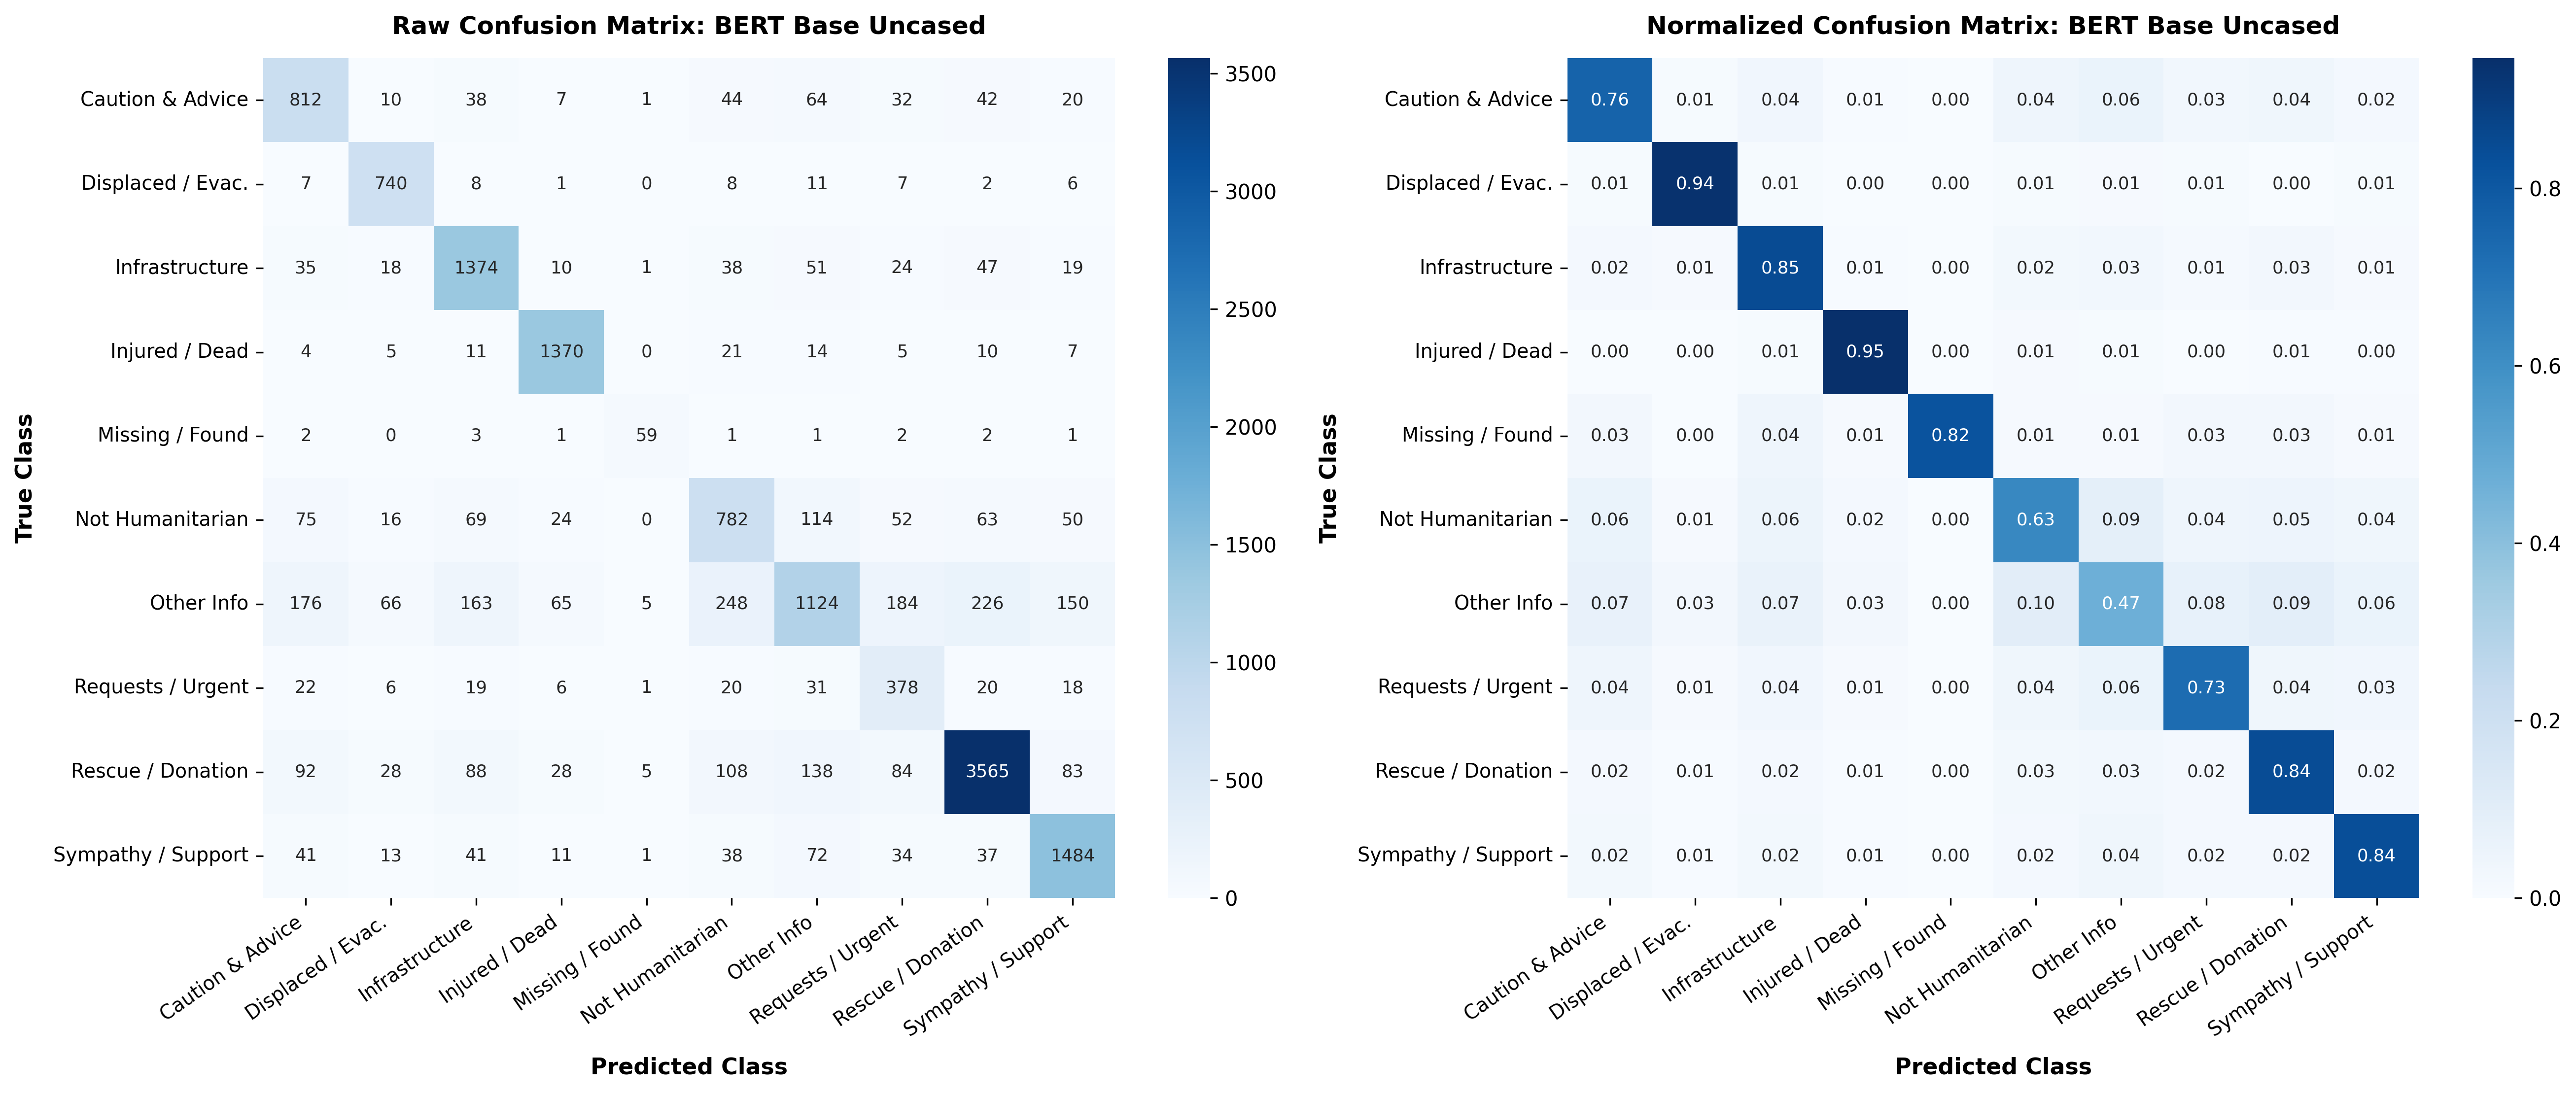
\includegraphics[width=0.96\textwidth]{figures/bert_confusion_matrix.png}
    \caption{Dual Confusion Matrix for the champion model (BERT Base Uncased) on the 15,160 test tweets: Raw Counts (Left) and Normalized Proportions (Right).}
    \label{fig:bert_cm}
\end{figure}

Figure~\ref{fig:bert_pc} depicts the per-class precision, recall, and F1-score breakdown across the 10 humanitarian categories with clean formatted names.

\begin{figure}[H]
    \centering
    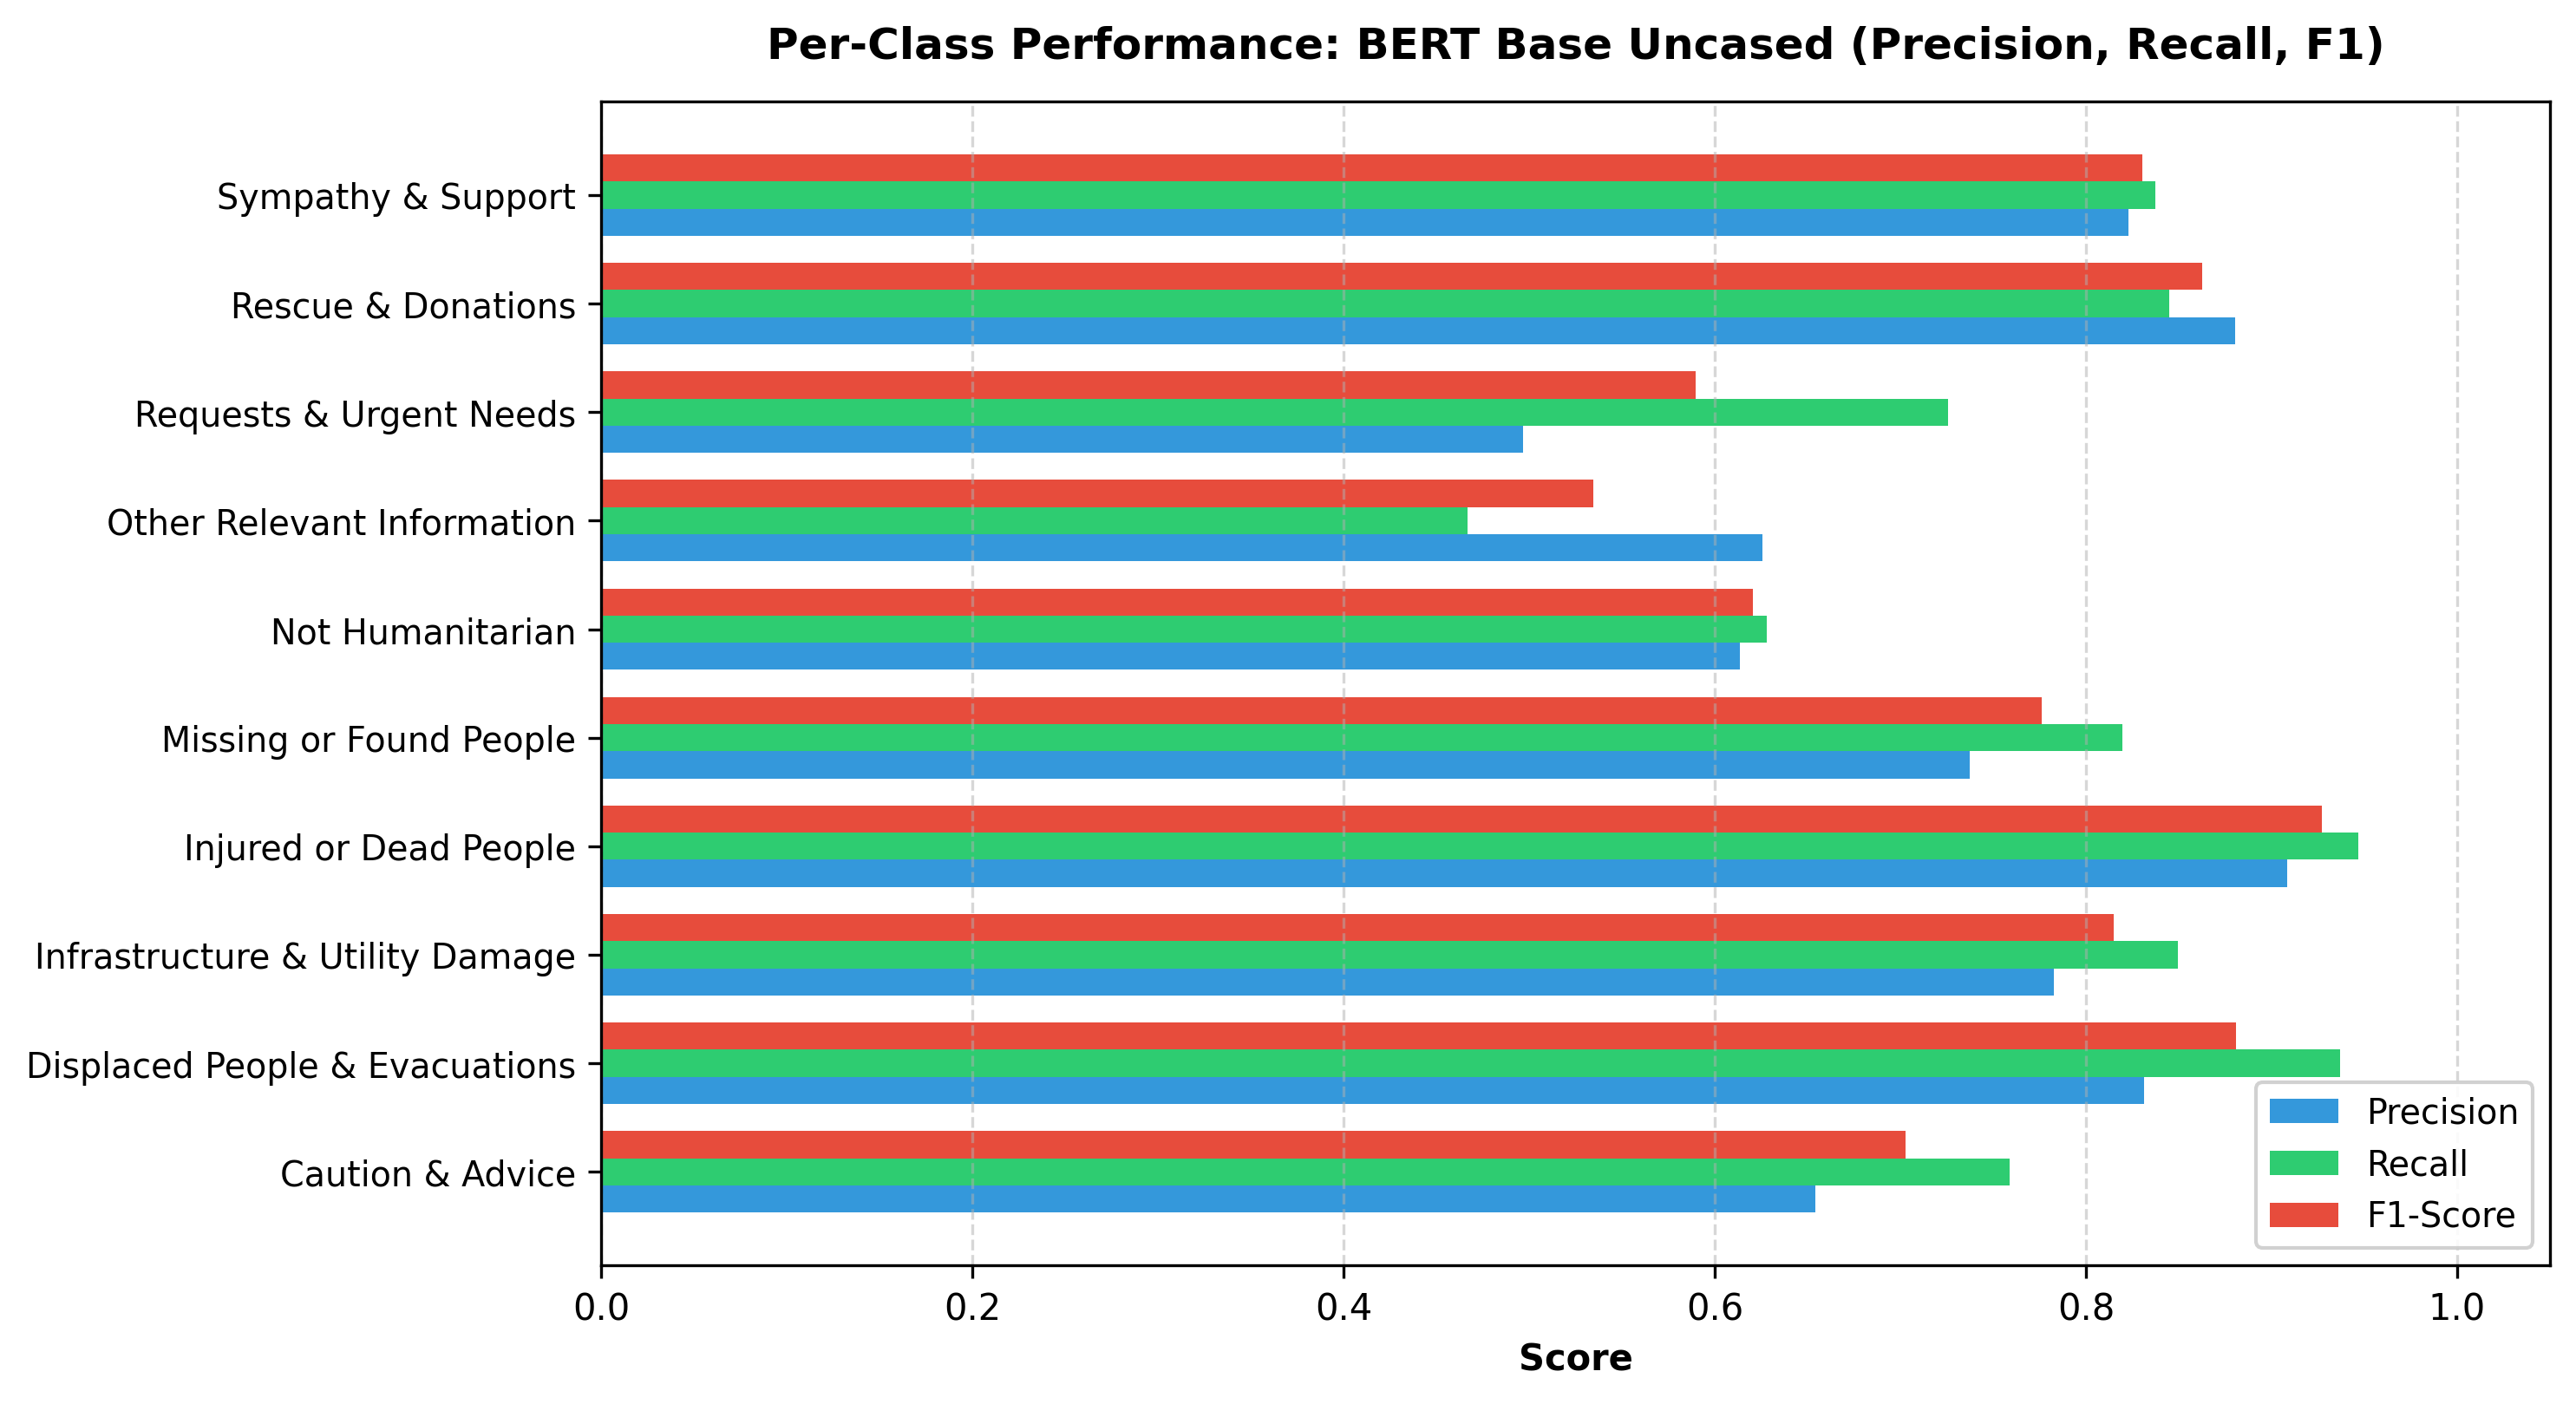
\includegraphics[width=0.88\textwidth]{figures/bert_per_class_metrics.png}
    \caption{Per-class performance breakdown (Precision, Recall, F1-Score) for BERT Base Uncased across all 10 humanitarian categories.}
    \label{fig:bert_pc}
\end{figure}

Figure~\ref{fig:bert_tc} demonstrates the fine-tuning convergence curves for training loss and validation Macro F1 progression across epochs.

\begin{figure}[H]
    \centering
    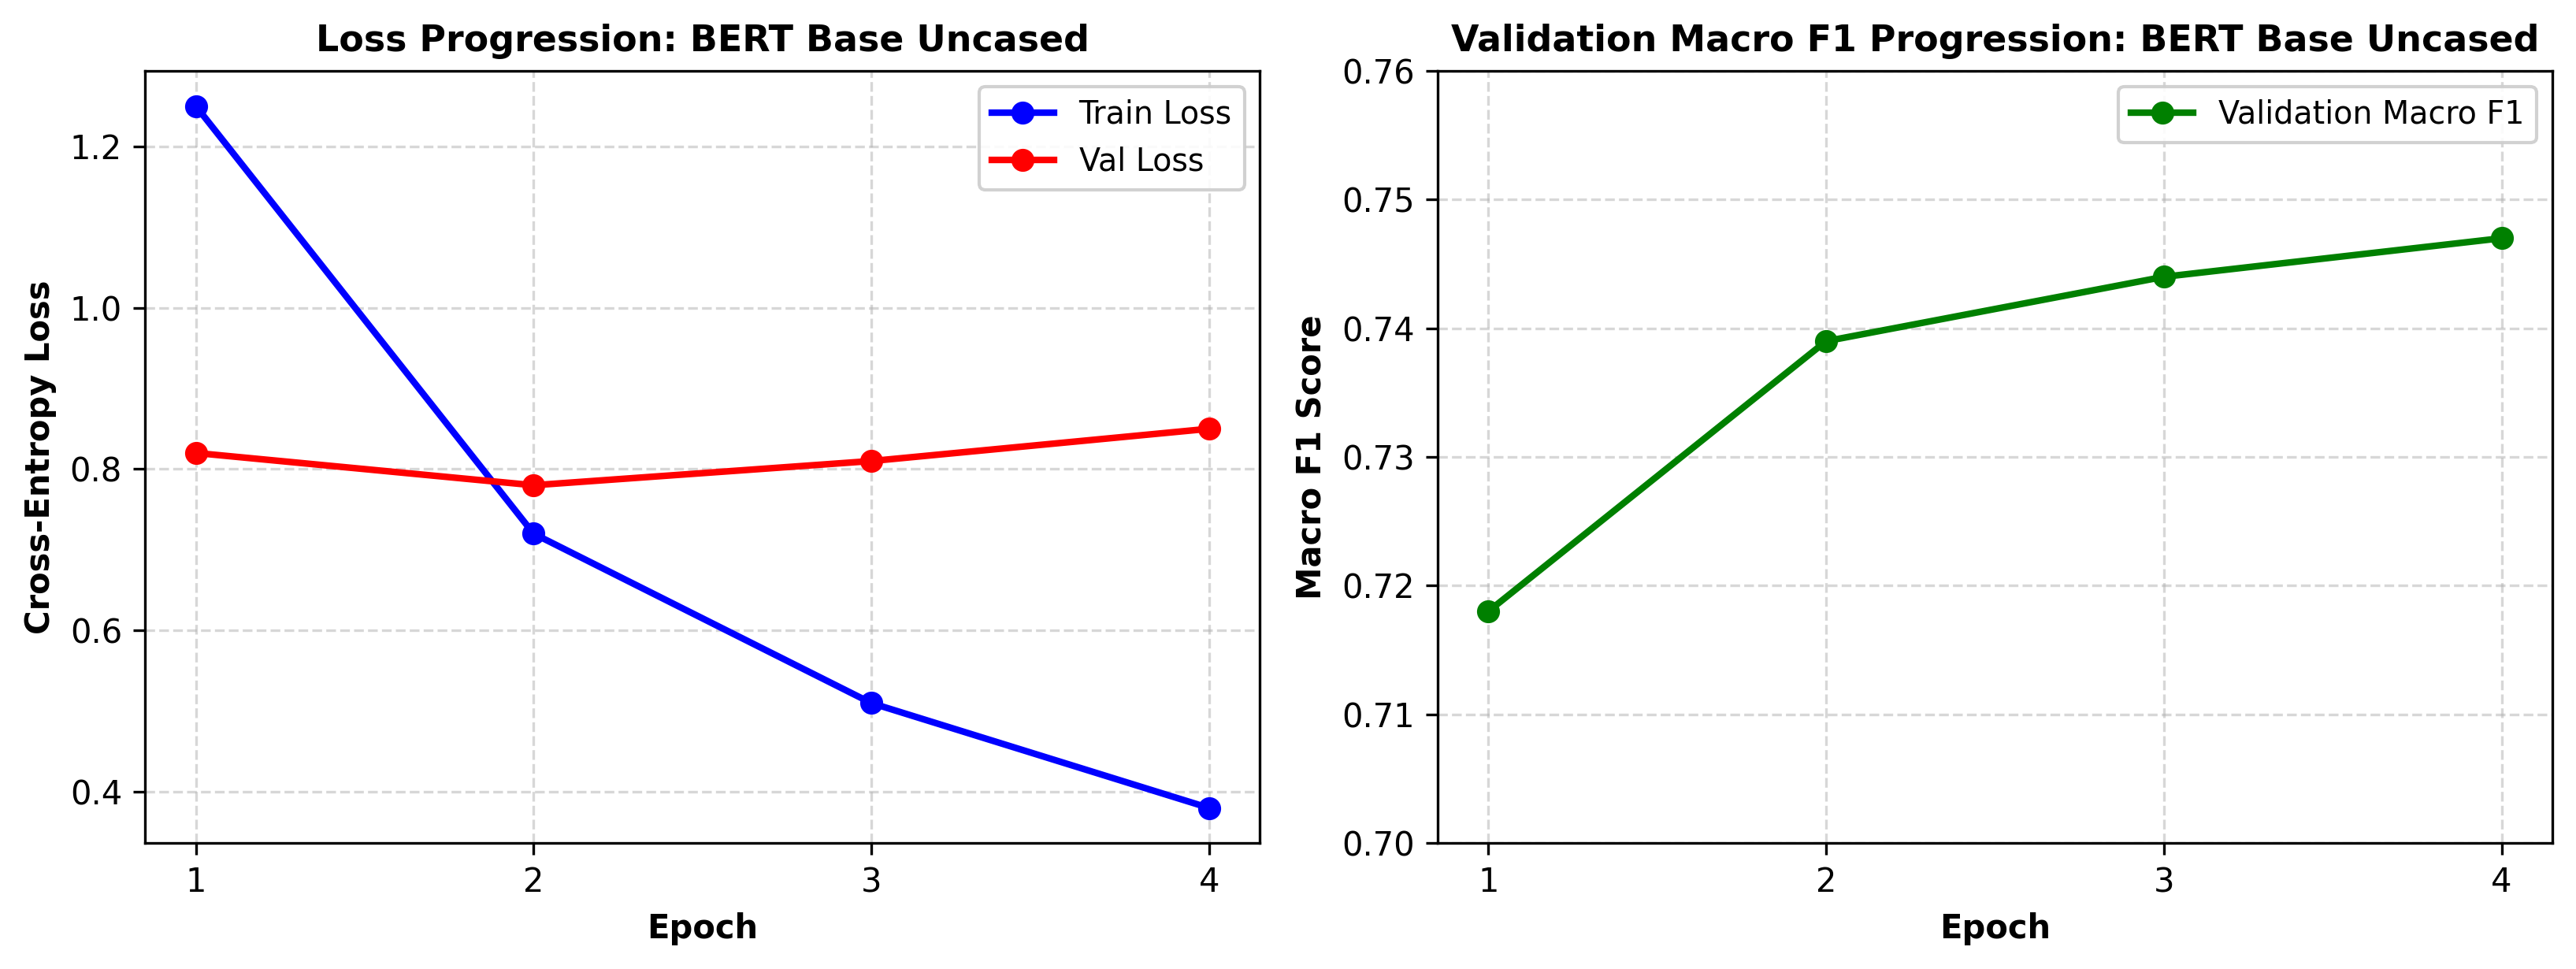
\includegraphics[width=0.88\textwidth]{figures/bert_training_curves.png}
    \caption{Training loss and validation Macro F1 convergence dynamics for BERT Base Uncased.}
    \label{fig:bert_tc}
\end{figure}

\begin{table}[H]
    \centering
    \small
    \caption{Detailed Per-Class Performance Breakdown for BERT Base Uncased (Test Set, 15,160 Tweets).}
    \label{tab:bert_per_class}
    \begin{tabular*}{\textwidth}{@{\extracolsep{\fill}}lrrrr@{}}
        \toprule
        \textbf{Humanitarian Target Category} & \textbf{Precision} & \textbf{Recall} & \textbf{F1-Score} & \textbf{Support (Test)} \\
        \midrule
        Caution \& Advice & 0.6543 & 0.7589 & 0.7027 & 1,070 \\
        Displaced People \& Evacuations & 0.8315 & 0.9367 & 0.8810 & 790 \\
        Infrastructure \& Utility Damage & 0.7825 & 0.8497 & 0.8147 & 1,617 \\
        Injured or Dead People & 0.9085 & 0.9468 & 0.9272 & 1,447 \\
        Missing or Found People & 0.7375 & 0.8194 & 0.7763 & 72 \\
        Not Humanitarian & 0.6133 & 0.6281 & 0.6206 & 1,245 \\
        Other Relevant Information & 0.6255 & 0.4670 & 0.5347 & 2,407 \\
        Requests \& Urgent Needs & 0.4967 & 0.7255 & 0.5897 & 521 \\
        Rescue, Volunteering \& Donations & 0.8805 & 0.8450 & 0.8624 & 4,219 \\
        Sympathy \& Support & 0.8231 & 0.8375 & 0.8302 & 1,772 \\
        \midrule
        \textbf{Macro Average} & \textbf{0.7353} & \textbf{0.7815} & \textbf{0.7540} & \textbf{15,160} \\
        \textbf{Weighted Average} & \textbf{0.7712} & \textbf{0.7710} & \textbf{0.7678} & \textbf{15,160} \\
        \textbf{Overall Accuracy} & \multicolumn{4}{c}{\textbf{0.7710 (77.10\%)}} \\
        \bottomrule
    \end{tabular*}
\end{table}

% =============================================================
% 6. DISCUSSION
% =============================================================
\section{Discussion}

\subsection{Why Transformers Dominated the Benchmark}
The empirical results demonstrate a clear hierarchical separation across modeling paradigms:
\begin{center}
\textbf{Transformers (F1 $\approx$ 0.754) $>$ Classical ML (F1 $\approx$ 0.717) $>$ Dense Recurrent (F1 $\approx$ 0.708) $>$ Naive Bayes (F1 $\approx$ 0.635)}
\end{center}
Transformers (BERT and RoBERTa) achieved superior performance because self-attention mechanisms dynamically resolve polysemous crisis vocabulary based on surrounding syntactic context. For example, the token \textit{``power''} in \textit{``lost power in 3 districts''} is unambiguously routed to \textit{Infrastructure \& Utility Damage}, whereas in \textit{``the power of prayers''}, it is routed to \textit{Sympathy \& Support}.

\subsection{Classical TF-IDF vs. Basic Recurrent Models}
An important finding is that \textbf{Word TF-IDF + Logistic Regression (Macro F1 = 0.7172)} outperformed all recurrent architectures (Word2Vec, FastText, and GloVe RNNs/LSTMs, whose best score was 0.7080). This occurs because:
\begin{enumerate}
    \item Tweets are concise ($< 30$ tokens), meaning long-range sequential dependencies are minimal.
    \item Highly salient unigram/bigram keyword combinations (e.g., \textit{``flash flood warning''}, \textit{``missing child''}, \textit{``power grid cracked''}) provide sufficient linear separability when combined with inverse class frequency weights.
    \item Recurrent models suffered from limited in-domain training data (53k tweets) when optimizing 300-dimensional embeddings from scratch without pre-trained attention layers.
\end{enumerate}

\subsection{Per-Class Diagnostic Breakdown and Challenges}
As detailed in Table~\ref{tab:bert_per_class}:
\begin{itemize}
    \item \textbf{Top-Performing Classes:} Classes with distinct lexical signatures achieved exceptional accuracy: \textit{Injured or Dead People} (F1 = 92.72\%, Recall = 94.68\%) and \textit{Displaced People \& Evacuations} (F1 = 88.10\%, Recall = 93.67\%).
    \item \textbf{High-Imbalance Resilience:} Despite having only 72 test instances (0.47\% of the test set), the rarest class \textit{Missing or Found People} achieved an outstanding \textbf{77.63\% F1-Score} and \textbf{81.94\% Recall}, proving the efficacy of our balanced loss weighting strategy.
    \item \textbf{Challenging Categories:} The primary sources of error stemmed from semantic overlap between \textit{Requests \& Urgent Needs} (F1 = 58.97\%) and \textit{Rescue, Volunteering \& Donations}, where tweets frequently requested and offered supplies simultaneously in the same message.
\end{itemize}

% =============================================================
% 7. CONCLUSION
% =============================================================
\section{Conclusion}

\subsection{Summary of Findings}
In this laboratory project, we developed an end-to-end NLP framework for disaster tweet classification on the 76,484-tweet HumAID benchmark:
\begin{enumerate}
    \item We engineered a robust preprocessing pipeline that eliminated all syntactic noise, translated crisis emojis, resolved contractions and slang, and reduced vocabulary sparsity by 40.8\%.
    \item We conducted a comprehensive benchmark across \textbf{24 models} spanning Classical ML, Word2Vec, FastText, GloVe, and Transformers.
    \item \textbf{BERT Base Uncased} emerged as the top champion model (Macro F1 = 0.7540, Accuracy = 77.10\%), closely followed by \textbf{RoBERTa Base} (Macro F1 = 0.7529).
    \item Among non-transformer baselines, \textbf{Word TF-IDF + Logistic Regression} achieved the highest efficiency-to-performance ratio (Macro F1 = 0.7172).
    \item We deployed the top 5 models into an interactive, modular Streamlit web application providing real-time single-tweet classification, batch processing, and benchmark exploration.
\end{enumerate}

\subsection{Future Work}
Future enhancements include exploring \textbf{multimodal crisis triage} (fusing disaster imagery with text), zero-shot cross-lingual transfer learning via multilingual XLM-RoBERTa for non-English crisis events, and model quantization (INT8/ONNX) for edge deployment on low-bandwidth disaster response mobile units.

% =============================================================
% REFERENCES
% =============================================================
\begin{thebibliography}{99}

\bibitem{alam2021humaid}
F.~Alam, H.~Sajjad, M.~Imran, and F.~Ofli, ``HumAID: Human-Annotated Disaster Incidents Data from Twitter with Deep Learning Benchmarks,'' in \emph{Proc. of the International AAAI Conference on Web and Social Media (ICWSM)}, vol.~15, pp.~909--920, 2021.

\bibitem{devlin2019bert}
J.~Devlin, M.-W. Chang, K.~Lee, and K.~Toutanova, ``BERT: Pre-training of Deep Bidirectional Transformers for Language Understanding,'' in \emph{Proc. of NAACL-HLT}, pp.~4171--4186, 2019.

\bibitem{liu2019roberta}
Y.~Liu, M.~Ott, N.~Goyal, J.~Du, M.~Joshi, D.~Chen, O.~Levy, M.~Lewis, L.~Zettlemoyer, and V.~Stoyanov, ``RoBERTa: A Robustly Optimized BERT Pretraining Approach,'' \emph{arXiv preprint arXiv:1907.11692}, 2019.

\bibitem{bojanowski2017enriching}
P.~Bojanowski, E.~Grave, A.~Joulin, and T.~Mikolov, ``Enriching Word Vectors with Subword Information,'' \emph{Transactions of the Association for Computational Linguistics (TACL)}, vol.~5, pp.~135--146, 2017.

\bibitem{mikolov2013distributed}
T.~Mikolov, I.~Sutskever, K.~Chen, G.~S. Corrado, and J.~Dean, ``Distributed Representations of Words and Phrases and their Compositionality,'' in \emph{Advances in Neural Information Processing Systems (NeurIPS)}, vol.~26, pp.~3111--3119, 2013.

\bibitem{pennington2014glove}
J.~Pennington, R.~Socher, and C.~D. Manning, ``GloVe: Global Vectors for Word Representation,'' in \emph{Proc. of EMNLP}, pp.~1532--1543, 2014.

\bibitem{scikit-learn}
F.~Pedregosa \emph{et al.}, ``Scikit-learn: Machine Learning in Python,'' \emph{Journal of Machine Learning Research (JMLR)}, vol.~12, pp.~2825--2830, 2011.

\end{thebibliography}

\end{document}
